\documentclass[oneside,14pt,a4paper]{extbook}
\usepackage{multicol}

\usepackage[T2A]{fontenc}
\usepackage[utf8]{inputenc}
\usepackage[english, russian]{babel}

%%% Поля и разметка страницы %%%
\usepackage{geometry}
\geometry{a4paper,top=2.0cm,bottom=2.0cm,left=2.5cm,right=1cm}

%%% Математические пакеты %%%
\usepackage{amsfonts,amsmath,amssymb,amsthm,mathtools}

%%% Оформление абзацев %%%
\usepackage{indentfirst}

%%% Цвета %%%
\usepackage{colortbl}

%%% Таблицы %%%
\usepackage{longtable}
\usepackage{multirow,makecell,array}
\usepackage{booktabs}

%%% Общее форматирование
\usepackage{soul}

%%% Гиперссылки %%%
\usepackage[linktocpage=true,plainpages=false,pdfpagelabels=false,colorlinks=true,urlcolor=black]{hyperref}
\hypersetup{
    colorlinks, linkcolor={black},
    citecolor={black}, urlcolor={black}
}

%%% Изображения %%%
\usepackage{graphicx}
\usepackage{pgfplots}
\pgfplotsset{compat=1.18}
\usepackage{tikz}
\usetikzlibrary{arrows,calc,fit,decorations.markings,positioning,shapes.geometric,shadows,trees,arrows.meta}

%%% Алгоритмы %%%
\usepackage{algorithm,algpseudocode}
\newcolumntype{H}{>{\setbox0=\hbox\bgroup}c<{\egroup}@{}}

%%% Оформление кода %%%
\usepackage{listings}

%%% Расположение объектов %%%
\usepackage{float}
\usepackage{caption}
\usepackage{subcaption}

%%% Комментарии %%%
\usepackage{comment}

%%% Доп. пакеты %%%
\usepackage{microtype}
\usepackage{relsize}
\usepackage[all]{xy}
\usepackage{pdfpages}
\usepackage{mdframed}

%%% Заголовки %%%
\usepackage{titlesec}
\titleformat{\chapter}[display]
  {\LARGE\bfseries}
  {\chaptertitlename\ \thechapter}{20pt}{\LARGE}
\titleformat{\section}
  {\Large\bfseries}
  {\thesection}{1em}{}

%%% Библиография (ГОСТ) %%%
\usepackage[style=gost-numeric]{biblatex}
\addbibresource{chapters/literature-review.bib}

%%% Стили страницы %%%
\makeatletter
\renewcommand{\@evenhead}{\vbox{\hbox to \textwidth {\hfil\thepage\hfil}}}
\renewcommand{\@oddhead}{\vbox{\hbox to \textwidth {\hfil\thepage\hfil}}}
\makeatother
\sloppy
\clubpenalty=10000
\widowpenalty=10000
\makeatletter
\renewcommand{\@biblabel}[1]{#1.}
\makeatother

%%% Теоремы %%%
\newtheorem{theorem}{Теорема}[chapter]
\newtheorem{definition}{Определение}[chapter]
\newtheorem{remark}{Замечание}[chapter]
\newtheorem{lemma}{Лемма}[chapter]

%%% Интервалы %%%
\linespread{1.3}
\parindent=1.25cm

%%% Todonotes %%%
\usepackage[colorinlistoftodos,textwidth=4cm,shadow]{todonotes}

\begin{document}

\tableofcontents

\addcontentsline{toc}{chapter}{Введение}
\chapter*{Введение}

Большие языковые модели (Large Language Models, LLM) стали одной из наиболее значимых технологий последнего десятилетия, трансформировав подходы к обработке естественного языка, генерации текста, машинному переводу и широкому спектру прикладных задач. Модели семейств GPT~\cite{radford2018gpt,radford2019gpt2,brown2020gpt3,achiam2023gpt4}, LLaMA~\cite{touvron2023llama}, Gemini~\cite{team2023gemini}, DeepSeek~\cite{deepseek2024v2} и GigaChat~\cite{2506.09440} демонстрируют способности, ранее считавшиеся недоступными для автоматических систем: связное рассуждение, следование сложным инструкциям, генерация программного кода и анализ мультимодальных данных.

Вместе с ростом возможностей и масштабов внедрения LLM в критически важные приложения возрастает актуальность исследования их безопасности. Мультимодальные модели, обрабатывающие одновременно текстовые и визуальные данные, открывают дополнительные поверхности атак, включая состязательные возмущения изображений, кросс-модальные атаки взлома и внедрение вредоносных инструкций через визуальный канал. Систематическое изучение уязвимостей и разработка защитных механизмов являются необходимым условием безопасного развёртывания данных технологий.

Ключевая гипотеза работы состоит в том, что безопасность мультимодальных LLM должна обеспечиваться не только фильтрацией входов и выходов, но и контролем информационного пространства, из которого модель получает внешние знания. Поэтому поисковый стек рассматривается как часть защитного контура: он ограничивает доступ модели к курируемым источникам, снижает галлюцинации и уменьшает риск генерации ответов на основе вредоносного или недостоверного контента.

%% =================================================================
\section*{Цель, задачи и научная новизна работы}
\addcontentsline{toc}{section}{Цель, задачи и научная новизна работы}
%% =================================================================

\textbf{Актуальность темы.} Промышленное развёртывание русскоязычных и мультимодальных LLM требует одновременно качественного информационного поиска (для заземления ответов на достоверных источниках) и надёжных механизмов безопасности (для сдерживания атак при сохранении полезности). Оба направления для русского языка существенно менее проработаны, чем для английского, а их интеграция в единый защитный контур в литературе систематически не рассматривалась.

\textbf{Целью} работы является разработка методов информационного поиска и переранжирования для русскоязычных больших языковых моделей, а также исследование их интеграции в конвейер безопасного развёртывания мультимодальных LLM через механизм курируемого безопасного поиска.

Для достижения поставленной цели в работе решаются следующие \textbf{задачи}:
\begin{enumerate}
    \item систематизировать современные подходы к построению текстовых и мультимодальных эмбеддингов, методы переранжирования, парадигмы генерации с извлечением информации (RAG), а также системы обеспечения безопасности и уязвимости мультимодальных моделей;
    \item разработать фреймворк обучения высокопроизводительных русскоязычных текстовых эмбеддингов на основе декодерной большой языковой модели и оценить его на бенчмарке MTEB(rus);
    \item предложить компактный реранкер для уточнения результатов первичного извлечения в двухэтапном конвейере поиска и экспериментально оценить его на русскоязычных IR-бенчмарках;
    \item построить поисковый стек, объединяющий лексический, плотный, гибридный и двухэтапный поиск, и обосновать преимущества RAG в части снижения галлюцинаций и устранения необходимости переобучения при обновлении данных;
    \item разработать двухэтапный конвейер обеспечения безопасности мультимодальных моделей, включающий потоковый классификатор обменов и безопасную модель, дообученную с подкреплением с наградой за безопасность;
    \item интегрировать разработанный поисковый стек в конвейер безопасности в виде инструмента безопасного поиска по курируемому индексу и предложить расширение защитных механизмов на визуальную модальность.
\end{enumerate}

\textbf{Объектом исследования} являются большие языковые и мультимодальные модели в контексте их безопасного развёртывания. \textbf{Предметом исследования} выступают методы информационного поиска (эмбеддинги, переранжирование, генерация с извлечением информации) и механизмы обеспечения безопасности, а также их интеграция в единый конвейер.

\textbf{Научная новизна} работы состоит в следующем:
\begin{enumerate}
    \item предложен иерархический трёхэтапный конвейер инструктивного дообучения декодерной LLM GigaChat для построения русскоязычных текстовых эмбеддингов, занявший первое место на русскоязычном бенчмарке MTEB(rus, v1.1)~\cite{2510.22369};
    \item разработан кросс-энкодер реранкер на основе компактных декодерных моделей GigaChat (0.6B и 3B), адаптирующий декодерную LLM к задаче переранжирования заменой каузального внимания на двунаправленное, агрегацией mean pooling и выделенной классификационной головой;
    \item предложен двухэтапный конвейер обеспечения безопасности, в котором независимый от защищаемой модели потоковый классификатор обменов на основе MoE-модели сочетается с безопасной моделью, дообученной с подкреплением с гибридной наградой за безопасность;
    \item впервые поисковый стек на основе эмбеддингов и переранжирования интегрирован в конвейер безопасности в виде инструмента безопасного поиска по курируемому индексу, обеспечивающего защищённой модели актуальный и достоверный взгляд на предметную область, а защитные механизмы распространены на визуальную модальность.
\end{enumerate}

\textbf{Практическая значимость} работы определяется применимостью предложенных методов в промышленных русскоязычных системах: модель эмбеддингов GigaEmbeddings и базовые модели семейства GigaChat выпущены в открытый доступ~\cite{2506.09440,2510.22369,gigaembeddings_hf,gigachat3_10b}, а предложенный конвейер обеспечения безопасности рассчитан на развёртывание с низкими накладными расходами и независимое обновление защитного слоя относительно защищаемой модели.

На \textbf{защиту выносятся} следующие положения:
\begin{enumerate}
    \item адаптация декодерной LLM к двунаправленному вниманию с латентным пулингом и трёхэтапным инструктивным дообучением позволяет получать русскоязычные эмбеддинги уровня state-of-the-art при более чем вдвое меньшем числе параметров ($\approx$3 млрд против 7--8 млрд у сильнейших базовых моделей);
    \item адаптация компактной декодерной LLM к задаче переранжирования (замена каузального внимания на двунаправленное, mean pooling, выделенная классификационная голова) обеспечивает качество уровня лучших открытых реранкеров сопоставимого размера на русскоязычных IR-бенчмарках;
    \item классификация на уровне обмена с пороговым правилом решения и независимостью от защищаемой модели обеспечивает эффективную модерацию контента, а гибридная награда за безопасность позволяет сохранять баланс между безопасностью и полезностью при обучении с подкреплением;
    \item интеграция поискового стека в конвейер безопасности в виде инструмента безопасного поиска по курируемому индексу объединяет преимущества RAG (достоверность, актуальность) с механизмами обеспечения безопасности в единой системе.
\end{enumerate}

\textbf{Личный вклад автора.} Семейство моделей GigaChat (Глава~\ref{ch:gigachat}) разработано коллективом авторов~\cite{2506.09440}; в настоящей работе оно используется как методологическая основа --- источник предобученных бэкбонов для последующих компонентов --- и не выносится на защиту в качестве самостоятельного результата. Фреймворк текстовых эмбеддингов GigaEmbeddings (Глава~\ref{ch:gigaembeddings}) разработан автором: архитектура, трёхэтапный конвейер обучения и экспериментальная оценка~\cite{2510.22369}. Кросс-энкодер реранкер (Глава~\ref{ch:reranking}) предложен и исследован в магистерской диссертации Е.\,А.~Краснопёрова, выполненной под со-руководством автора; автору принадлежат постановка задачи, выбор архитектурного направления и научное руководство, экспериментальная реализация выполнена магистрантом. Поисковый стек (Глава~\ref{ch:rag}) и двухэтапный конвейер обеспечения безопасности (Глава~\ref{ch:safety}), включая модель угроз, потоковый классификатор обменов, дизайн награды за безопасность и интеграцию инструмента безопасного поиска, разработаны автором.

\textbf{Апробация результатов.} Основные результаты работы опубликованы в статьях, посвящённых семейству моделей GigaChat~\cite{2506.09440} и фреймворку GigaEmbeddings~\cite{2510.22369}. Модель эмбеддингов и базовые модели семейства GigaChat выпущены в открытый доступ~\cite{gigaembeddings_hf,gigachat3_10b}; модель GigaEmbeddings по состоянию на июнь 2026~г. занимает первое место в публичном рейтинге MTEB(rus, v1.1).

Соответствие решаемых задач главам диссертации и полученным результатам приведено в Таблице~\ref{tab:intro_map}.

\begin{table}[H]
    \centering
    \caption{Соответствие <<задача~--- глава~--- результат>>.}
    \label{tab:intro_map}
    \begin{tabular}{p{0.26\textwidth}p{0.12\textwidth}p{0.50\textwidth}}
        \toprule
        Задача & Глава & Результат \\
        \midrule
        Обзор методов & Глава~\ref{ch:lit_review} & систематизация направлений: эмбеддинги, переранжирование, RAG, безопасность \\
        Эмбеддинги (GigaEmbeddings) & Глава~\ref{ch:gigaembeddings} & первое место на MTEB(rus, v1.1), средний балл 74.16 \\
        Реранкер & Глава~\ref{ch:reranking} & nDCG@10 $0.78$ на RuBQ; лучшее качество среди открытых моделей сопоставимого размера \\
        RAG-стек & Глава~\ref{ch:rag} & лексический + плотный + гибридный (RRF) + двухэтапный поиск \\
        Конвейер безопасности & Глава~\ref{ch:safety} & потоковый классификатор обменов ($\mathrm{AUC}=0.83$ против $0.60$ у классификатора запросов) \\
        Безопасный индекс & Глава~\ref{ch:safety} & инструмент безопасного поиска по курируемому индексу (заземлённые ответы) \\
        \bottomrule
    \end{tabular}
\end{table}

%% =================================================================
\section*{Теоретические основы}
\addcontentsline{toc}{section}{Теоретические основы}
%% =================================================================

Настоящий раздел кратко вводит понятия, на которых строится изложение; детальный обзор методов вынесен в Главу~\ref{ch:lit_review}.

\textbf{Языковое моделирование.} Языковая модель оценивает вероятностное распределение над последовательностями токенов, $P(w_1,\ldots,w_n) = \prod_{i=1}^{n} P(w_i \mid w_1,\ldots,w_{i-1})$. Классические $n$-граммные модели со сглаживанием~\cite{chen1999empirical} ограничены фиксированным контекстом и разреженностью данных. Переход к нейронным моделям~\cite{bengio2003neural} и рекуррентным сетям --- RNN~\cite{mikolov2010recurrent}, LSTM~\cite{hochreiter1997lstm}, GRU~\cite{cho2014gru} --- позволил моделировать длинные зависимости, однако их последовательная природа ограничивала параллелизацию и масштабирование.

\textbf{Архитектура Transformer.} Предложенная Vaswani et al.~\cite{vaswani2017attention} архитектура (Рисунок~\ref{fig:transformer}) отказалась от рекуррентных вычислений в пользу механизма масштабированного скалярного произведения внимания $\mathrm{Attention}(\mathbf{Q}, \mathbf{K}, \mathbf{V}) = \mathrm{softmax}(\mathbf{Q}\mathbf{K}^\top / \sqrt{d_k})\,\mathbf{V}$, обеспечив параллелизацию обучения и моделирование зависимостей произвольной дальности. Современные модели применяют вращательное позиционное кодирование (RoPE)~\cite{su2024rope} и сформировали три парадигмы предобучения: энкодерную (BERT~\cite{devlin2019bert}), декодерную (GPT~\cite{radford2018gpt,radford2019gpt2,brown2020gpt3}) и энкодер-декодерную (T5~\cite{raffel2020t5}); среди фронтирных LLM доминирует декодерная архитектура благодаря масштабируемости и способности к обучению в контексте (in-context learning).

\begin{figure}[htbp]
    \centering
    \resizebox{0.55\textwidth}{!}{
        \usetikzlibrary{positioning, fit, shapes.geometric, arrows.meta, shadows, calc}

\begin{tikzpicture}[
    node distance=0.8cm and 1cm,
    layer/.style={
        draw,
        rectangle,
        rounded corners,
        minimum width=3cm,
        minimum height=1cm,
        align=center,
        fill=white,
        drop shadow
    },
    process/.style={
        draw,
        rectangle,
        rounded corners,
        minimum width=2.5cm,
        minimum height=0.8cm,
        align=center,
        fill=blue!10
    },
    arrow/.style={
        ->,
        >=Stealth,
        thick
    },
    addnorm/.style={
        draw,
        rectangle,
        rounded corners,
        minimum width=3cm,
        minimum height=0.6cm,
        fill=yellow!20,
        align=center,
        font=\small
    }
]

% Encoder Stack
\node[font=\bfseries] (input) {Inputs};
\node[process, above=0.5cm of input] (emb) {Input Embedding};
\node[circle, draw, fill=white, above=0.3cm of emb] (plus1) {+};
\node[right=0.5cm of plus1] (pos) {Positional Encoding};

\node[layer, fill=orange!20, above=0.5cm of plus1] (mha) {Multi-Head\\Attention};
\node[addnorm, above=0.3cm of mha] (norm1) {Add \& Norm};

\node[layer, fill=blue!10, above=0.5cm of norm1] (ffn) {Feed Forward};
\node[addnorm, above=0.3cm of ffn] (norm2) {Add \& Norm};

% Decoder Stack
\node[right=4cm of input, font=\bfseries, align=center] (output) {Outputs\\(shifted right)};
\node[process, above=0.5cm of output] (outemb) {Output Embedding};
\node[circle, draw, fill=white, above=0.3cm of outemb] (plus2) {+};
\node[right=0.5cm of plus2] (pos2) {Positional Encoding};

\node[layer, fill=orange!20, above=0.5cm of plus2] (mmha) {Masked\\Multi-Head Attention};
\node[addnorm, above=0.3cm of mmha] (norm3) {Add \& Norm};

\node[layer, fill=orange!20, above=0.5cm of norm3] (mha2) {Multi-Head\\Attention};
\node[addnorm, above=0.3cm of mha2] (norm4) {Add \& Norm};

\node[layer, fill=blue!10, above=0.5cm of norm4] (ffn2) {Feed Forward};
\node[addnorm, above=0.3cm of ffn2] (norm5) {Add \& Norm};

\node[process, fill=green!10, above=0.5cm of norm5] (linear) {Linear};
\node[process, fill=green!20, above=0.3cm of linear] (softmax) {Softmax};
\node[above=0.3cm of softmax, font=\bfseries] (probs) {Output Probabilities};

% Connections Encoder
\draw[arrow] (input) -- (emb);
\draw[arrow] (emb) -- (plus1);
\draw[arrow] (pos) -- (plus1);
\draw[arrow] (plus1) -- (mha);
\draw[arrow] (mha) -- (norm1);
\draw[arrow] (norm1) -- (ffn);
\draw[arrow] (ffn) -- (norm2);

% Connections Decoder
\draw[arrow] (output) -- (outemb);
\draw[arrow] (outemb) -- (plus2);
\draw[arrow] (pos2) -- (plus2);
\draw[arrow] (plus2) -- (mmha);
\draw[arrow] (mmha) -- (norm3);
\draw[arrow] (norm3) -- (mha2);
\draw[arrow] (mha2) -- (norm4);
\draw[arrow] (norm4) -- (ffn2);
\draw[arrow] (ffn2) -- (norm5);
\draw[arrow] (norm5) -- (linear);
\draw[arrow] (linear) -- (softmax);
\draw[arrow] (softmax) -- (probs);

% Cross Attention
\draw[arrow] (norm2.north) -- ++(0,0.2) -| (mha2.west);
\draw[arrow] (norm2.north) -- ++(0,0.2) -| (mha2.west); % Simplified, normally K, V

% Residuals (simplified visualization)
\draw[arrow, dashed] (plus1.west) -- ++(-0.5,0) |- (norm1.west);
\draw[arrow, dashed] (norm1.west) -- ++(-0.5,0) |- (norm2.west);

\draw[arrow, dashed] (plus2.east) -- ++(0.5,0) |- (norm3.east);
\draw[arrow, dashed] (norm3.east) -- ++(0.5,0) |- (norm4.east);
\draw[arrow, dashed] (norm4.east) -- ++(0.5,0) |- (norm5.east);

% Labels
\node[draw, dashed, fit=(mha) (norm2), label=left:N$\times$] (enc_block) {};
\node[draw, dashed, fit=(mmha) (norm5), label=right:N$\times$] (dec_block) {};

\node[below=0.1cm of enc_block, font=\bfseries] {Encoder};
\node[below=0.1cm of dec_block, font=\bfseries] {Decoder};

\end{tikzpicture}

    }
    \caption{Архитектура Transformer.}
    \label{fig:transformer}
\end{figure}

\textbf{Mixture of Experts.} Концепция смеси экспертов (Mixture of Experts, MoE)~\cite{jacobs1991moe,shazeer2017moe} реализует принцип условных вычислений (Рисунок~\ref{fig:moe_architecture}): для каждого токена обучаемый маршрутизатор активирует лишь $k \ll N$ экспертов из $N$, что позволяет существенно увеличить ёмкость модели без пропорционального роста вычислительных затрат. Слои MoE заменяют стандартные блоки прямого распространения (FFN), оставляя слой самовнимания без изменений. Подход масштабирован в GShard~\cite{lepikhin2021gshard} (600 млрд параметров) и Switch Transformers~\cite{fedus2022switch} (ускорение предобучения до 7 раз) и лежит в основе Mixtral~\cite{jiang2024mixtral}, DeepSeek~\cite{deepseek2024v2,dai2024deepseekmoe} и GigaChat~\cite{2506.09440}, подробно рассматриваемого в Главе~\ref{ch:gigachat}. Основными вызовами остаются балансировка нагрузки между экспертами и повышенные требования к памяти.

\begin{figure}[htbp]
    \centering
    \resizebox{0.8\textwidth}{!}{
        \usetikzlibrary{positioning, shapes.geometric, arrows.meta, shadows, calc}

\begin{tikzpicture}[
    node distance=1cm and 1.2cm,
    block/.style={
        draw,
        rectangle,
        rounded corners,
        minimum width=2cm,
        minimum height=1cm,
        align=center,
        drop shadow
    },
    expert/.style={
        draw,
        rectangle,
        rounded corners,
        minimum width=1.8cm,
        minimum height=1cm,
        align=center,
        drop shadow
    },
    arrow/.style={
        ->,
        >=Stealth,
        thick
    },
    activearrow/.style={
        ->,
        >=Stealth,
        line width=1.2pt,
        blue!70
    },
    inactivearrow/.style={
        ->,
        >=Stealth,
        thick,
        densely dashed,
        draw=gray!50
    }
]

% Input
\node[block, fill=gray!10] (input) {$\mathbf{x}$\\(Input Token)};

% Router
\node[block, fill=orange!20, above=1.2cm of input] (router) {Gating Network\\(Router)};

% Experts row
\node[expert, fill=blue!25, above left=1.5cm and 3.5cm of router] (e1) {Expert 1\\(FFN)};
\node[expert, fill=gray!8, draw=gray!40, right=0.8cm of e1] (e2) {\color{gray!60}Expert 2\\(FFN)};
\node[expert, fill=blue!25, right=0.8cm of e2] (e3) {Expert 3\\(FFN)};
\node[right=0.6cm of e3, font=\Large] (dots) {$\cdots$};
\node[expert, fill=gray!8, draw=gray!40, right=0.6cm of dots] (en) {\color{gray!60}Expert $N$\\(FFN)};

% Weighted sum
\node[block, fill=green!15, above=1.5cm of router |- e1.north, xshift=4.35cm] (sum) {$\displaystyle\sum_{i} G(\mathbf{x})_i \cdot E_i(\mathbf{x})$};

% Output
\node[block, fill=gray!10, above=1cm of sum] (output) {$\mathbf{y}$\\(Output)};

% Input to Router
\draw[arrow] (input) -- (router);

% Router to active experts
\draw[activearrow] (router.north) -- ++(0, 0.4) -| (e1.south)
    node[pos=0.75, left, font=\small, text=blue!70] {$g_1$};
\draw[activearrow] (router.north) -- ++(0, 0.4) -| (e3.south)
    node[pos=0.75, left, font=\small, text=blue!70] {$g_3$};

% Router to inactive experts (dashed, no arrowhead)
\draw[densely dashed, gray!50, thick] (router.north) -- ++(0, 0.4) -| (e2.south);
\draw[densely dashed, gray!50, thick] (router.north) -- ++(0, 0.4) -| (en.south);

% Active experts to weighted sum
\draw[activearrow] (e1.north) -- ++(0, 0.5) -| ([xshift=-0.6cm]sum.south);
\draw[activearrow] (e3.north) -- ++(0, 0.8) -| ([xshift=0.6cm]sum.south);

% Weighted sum to output
\draw[arrow] (sum) -- (output);

% Annotations
\node[right=0.5cm of router, font=\small, text=black!70, align=left] (annot) {Top-$k$ selection\\($k = 2$ in this example)};


\end{tikzpicture}

    }
    \caption{Архитектура разреженного слоя Mixture of Experts. Маршрутизатор (gating network) для каждого входного токена выбирает подмножество экспертов (top-$k$); неактивные эксперты показаны пунктиром.}
    \label{fig:moe_architecture}
\end{figure}

\textbf{Современные и мультимодальные модели.} Развитие LLM в 2017--2026~гг. обусловлено ростом объёма данных, вычислительных мощностей и числа параметров. Классические законы масштабирования Kaplan et al.~\cite{kaplan2020scaling} и Hoffmann et al. (Chinchilla)~\cite{hoffmann2022chinchilla} установили степенные зависимости качества от вычислительного бюджета; при обучении современных моделей, однако, на исходные Chinchilla-законы ориентируются всё реже, уступая место законам масштабирования пост-обучения, инференса и вычислений на этапе вывода (test-time compute), а также законам масштабирования архитектуры MoE. Открытые модели LLaMA~\cite{touvron2023llama,touvron2023llama2,grattafiori2024llama3}, Mistral~7B~\cite{jiang2023mistral} (с группированным запросным вниманием, GQA), Qwen~\cite{bai2023qwen} и DeepSeek~\cite{deepseek2024v2} (с латентным вниманием, MLA) обеспечивают воспроизводимость исследований. Мультимодальные LLM (MLLM, Рисунок~\ref{fig:multimodal_llm}) объединяют визуальный энкодер (например, ViT~\cite{dosovitskiy2020vit}), адаптер и декодерную LLM (GPT-4V~\cite{achiam2023gpt4}, Gemini~\cite{team2023gemini}, LLaVA~\cite{liu2024llava}); именно они являются основным объектом исследования, поскольку визуальный канал создаёт принципиально новые поверхности атак. Особую значимость для работы представляют русскоязычные модели --- GigaChat~\cite{2506.09440} и разработанный автором фреймворк текстовых эмбеддингов GigaEmbeddings~\cite{2510.22369}.

\begin{figure}[htbp]
    \centering
    \resizebox{0.8\textwidth}{!}{
        \usetikzlibrary{positioning, shapes.geometric, arrows.meta, shadows, calc}

\begin{tikzpicture}[
    block/.style={
        draw,
        rectangle,
        rounded corners,
        minimum width=2.8cm,
        minimum height=1cm,
        align=center,
        drop shadow
    },
    arrow/.style={
        ->,
        >=Stealth,
        thick
    }
]

% Row 1 (y=0): Image processing path
\node[block, fill=gray!10]    at (0,0)   (image) {Image};
\node[block, fill=orange!15]  at (4.5,0) (venc)  {Vision Encoder\\(ViT / CLIP)};
\node[block, fill=blue!10]    at (9,0)   (proj)  {Projection Layer\\(Adapter / MLP)};

% Row 2 (y=-2.5): Text path
\node[block, fill=gray!10]    at (0,-2.5) (text)   {Text Prompt};
\node[block, fill=blue!10]    at (4.5,-2.5) (tokemb) {Tokenizer +\\Embedding};

% LLM block centered between rows
\node[block, fill=purple!12, minimum width=3.2cm, minimum height=3.2cm]
    at (17.5,-1.25) (llm) {Large Language\\Model (Decoder)};

% Output
\node[block, fill=green!12] at (21.5,-1.25) (output) {Generated\\Response};

% Arrows — image path
\draw[arrow] (image) -- (venc);
\draw[arrow] (venc)  -- (proj);
\draw[arrow] (proj.east) -- (llm.west |- proj.east)
    node[midway, above, font=\small] {Visual Tokens};

% Arrows — text path
\draw[arrow] (text) -- (tokemb);
\draw[arrow] (tokemb.east) -- (llm.west |- tokemb.east)
    node[midway, above, font=\small] {Text Tokens};

% Arrow — output
\draw[arrow] (llm) -- (output);

\end{tikzpicture}

    }
    \caption{Архитектура мультимодальной большой языковой модели.}
    \label{fig:multimodal_llm}
\end{figure}

\textbf{Структура работы.} Глава~\ref{ch:lit_review} содержит обзор литературы, систематизирующий основные направления исследований: текстовые и мультимодальные эмбеддинги, методы переранжирования, системы генерации с извлечением информации (RAG), системы обеспечения безопасности ИИ и уязвимости мультимодальных моделей. Глава~\ref{ch:gigachat} посвящена семейству русскоязычных языковых моделей GigaChat, основанных на архитектуре Mixture of Experts, и вводит архитектурную и экспериментальную основу для последующих компонентов. Глава~\ref{ch:gigaembeddings} представляет фреймворк GigaEmbeddings для обучения высокопроизводительных текстовых эмбеддингов на основе декодерной LLM GigaChat-3B. Глава~\ref{ch:reranking} посвящена переранжированию в двухэтапном конвейере поиска и представляет авторский кросс-энкодер реранкер на основе компактных декодерных моделей GigaChat-0.6B и GigaChat-3B. Глава~\ref{ch:rag} рассматривает генерацию с извлечением информации, включая лексический (BM25), гибридный и двухэтапный поиск. Глава~\ref{ch:safety} объединяет результаты предшествующих глав в двухэтапном конвейере обеспечения безопасности мультимодальных моделей, включающем классификатор на основе GigaChat-10B MoE, безопасную модель, дообученную с подкреплением с наградой за безопасность, и инструмент безопасного поиска по курируемому индексу.


\chapter{Обзор литературы}\label{ch:lit_review}

В данной главе представлен обзор основных направлений исследований, связанных с проблемами безопасности больших языковых моделей в мультимодальном сценарии. Рассматриваются ключевые технологии, лежащие в основе современных систем обработки естественного языка: текстовые эмбеддинги, методы переранжирования, подходы генерации с извлечением информации (RAG), а также системы обеспечения безопасности и уязвимости мультимодальных моделей.

%% =================================================================
\section{Эмбеддинги текста}\label{sec:embeddings}
%% =================================================================

Текстовые эмбеддинги --- векторные представления текстовых фрагментов в непрерывном пространстве --- являются фундаментальным компонентом современных систем информационного поиска, кластеризации и классификации. Развитие данного направления прошло путь от классических методов, основанных на архитектуре BERT, до современных подходов, использующих большие языковые модели в качестве основы для получения универсальных представлений.

\subsection{Классические методы}\label{subsec:classic_embeddings}

Одной из первых работ, предложивших эффективный метод получения предложенческих эмбеддингов, стала Sentence-BERT (SBERT)~\cite{1908.10084}. Авторы использовали сиамскую и триплетную архитектуры поверх предобученной модели BERT для получения семантически осмысленных представлений предложений, допускающих сравнение с помощью косинусного сходства. Данный подход сократил время поиска наиболее похожей пары среди 10\,000 предложений с 65 часов до примерно 5 секунд при сохранении точности уровня BERT.

SimCSE~\cite{2104.08821} предложил простой, но эффективный метод контрастивного обучения предложенческих эмбеддингов. В ненаблюдаемом варианте модель использует dropout в качестве минимального возмущения данных: одно и то же предложение пропускается через энкодер дважды с различными масками dropout, образуя позитивные пары. Данный подход продемонстрировал значительное улучшение качества на задачах семантического текстового сходства.

DiffCSE~\cite{2204.10298} развил идеи SimCSE, предложив контрастивное обучение, основанное на различиях: модель обучается быть чувствительной к разнице между исходным предложением и его отредактированной версией, что позволяет лучше улавливать семантические нюансы.

\subsection{Модели на основе больших языковых моделей}\label{subsec:llm_embeddings}

С ростом масштаба языковых моделей исследователи обнаружили, что декодерные архитектуры, изначально предназначенные для генерации текста, могут быть успешно адаптированы для построения высококачественных эмбеддингов.

E5~\cite{2212.03533} представил семейство моделей текстовых эмбеддингов, обучаемых контрастивным методом на большом корпусе слабо размеченных текстовых пар (CCPairs). E5 стала первой моделью, превзошедшей сильную базовую линию BM25 на бенчмарке BEIR без использования размеченных данных. Дальнейшее развитие --- E5-Mistral~\cite{2401.00368} --- предложило получать высококачественные текстовые эмбеддинги с использованием исключительно синтетических данных, сгенерированных большими языковыми моделями для сотен тысяч задач на 93 языках, с последующей дообучкой декодерных моделей с открытым кодом.

GTE~\cite{2308.03281} применил многоэтапное контрастивное обучение для построения универсальных текстовых эмбеддингов, включая этапы ненаблюдаемого предобучения и наблюдаемой дообучки. BGE~\cite{2309.07597} предложил комплект ресурсов для развития китайских эмбеддингов общего назначения, включая предобученные модели, корпуса для дообучки и интегрированные кросс-энкодеры.

NV-Embed~\cite{2405.17428} представил архитектурные и методологические инновации для обучения LLM в качестве универсальных моделей эмбеддингов. Ключевые нововведения включают слой латентного внимания для пулинга, удаление каузальной маски внимания во время контрастивного обучения и двухэтапную процедуру обучения с инструкциями. Модели NV-Embed-v1 и NV-Embed-v2 заняли первое место в рейтинге MTEB.

AnglE~\cite{2309.12871} предложил оптимизацию текстовых эмбеддингов в угловом пространстве, что позволяет эффективнее разделять семантически близкие и далёкие тексты. Gecko~\cite{2403.20327} применил дистилляцию знаний из больших языковых моделей для создания компактных, но выразительных текстовых эмбеддингов.

ULLME~\cite{2408.03402} разработал унифицированный фреймворк для получения эмбеддингов из LLM с обучением, усиленным генерацией, что позволяет адаптировать произвольную языковую модель для задач построения представлений. Nomic Embed~\cite{2402.01613} представил воспроизводимый эмбеддер для длинных контекстов с открытым кодом.

Matryoshka Representation Learning~\cite{2205.13147} предложил метод обучения, при котором одна модель способна генерировать эмбеддинги различной размерности, допуская адаптивный выбор длины вектора в зависимости от вычислительных ограничений без существенной потери качества.

Среди наиболее современных подходов следует отметить Qwen3 Embedding~\cite{2506.05176}, основанный на фундаментальных моделях серии Qwen3 и продемонстрировавший передовые результаты как в задачах построения эмбеддингов, так и в переранжировании. Llama-Embed-Nemotron-8B~\cite{2511.07025} представляет универсальную модель текстовых эмбеддингов для многоязычных и кросс-языковых задач. KaLM-Embedding-V2~\cite{2506.20923} применил улучшенные методы обучения и курирования данных. Gemini Embedding~\cite{2503.07891} предложил обобщаемые эмбеддинги на основе моделей семейства Gemini. EmbeddingGemma~\cite{2509.20354} сфокусирован на создании мощных, но компактных текстовых представлений. Diffusion-Pretrained Dense and Contextual Embeddings~\cite{2602.11151} исследовал возможности диффузионного предобучения для получения плотных и контекстных эмбеддингов.

В работе GigaEmbeddings~\cite{2510.22369} представлен фреймворк для обучения высокопроизводительных русскоязычных текстовых эмбеддингов на основе иерархического инструктивного дообучения декодерной LLM (GigaChat-3B). Трёхэтапный конвейер, включающий масштабное контрастивное предобучение, дообучку с жёсткими негативными примерами и мультизадачную генерализацию, позволил достичь результатов уровня state-of-the-art на бенчмарке ruMTEB (69.1 среднего балла).

\subsection{Мультимодальные эмбеддинги и поиск}\label{subsec:multimodal_embeddings}

С развитием мультимодальных моделей возникла потребность в эмбеддингах, способных работать одновременно с текстовыми и визуальными данными.

MM-Embed~\cite{2411.02571} предложил подход к универсальному мультимодальному поиску на основе мультимодальных LLM, позволяющий обрабатывать запросы и документы, содержащие произвольные комбинации текста и изображений. MetaEmbed~\cite{2509.18095} представил метод масштабирования мультимодального поиска на этапе инференса с использованием гибкого позднего взаимодействия, что обеспечивает адаптивность к различным типам запросов.

CoMa~\cite{2511.08480} предложил эффективную парадигму предобучения мультимодальных эмбеддингов <<сжатие, затем сопоставление>>, что позволяет существенно снизить вычислительные затраты. MCA~\cite{2510.15543} сфокусирован на осведомлённости о составе модальностей для робастного композитного мультимодального поиска. MRMR~\cite{2510.09510} представил реалистичный мультидисциплинарный бенчмарк экспертного уровня для оценки мультимодального поиска, требующего глубокого рассуждения.

\subsection{Обзоры и бенчмарки эмбеддингов}\label{subsec:embedding_surveys}

Систематизация результатов в области текстовых эмбеддингов осуществлена в ряде обзорных работ. MTEB (Massive Text Embedding Benchmark)~\cite{2210.07316} предложил стандартизованный бенчмарк из 56 задач для всесторонней оценки моделей текстовых эмбеддингов, ставший де-факто стандартом в сообществе. Обзор \cite{2412.09165} представил всестороннее исследование на стыке текстовых эмбеддингов и больших языковых моделей, систематизировав методы обучения, архитектурные решения и области применения. Работа \cite{2406.01607} содержит анализ наиболее успешных методов на бенчмарке MTEB, выявляя ключевые факторы качества. Сравнительное исследование диффузионных и авторегрессионных языковых моделей с точки зрения текстовых эмбеддингов проведено в~\cite{2505.15045}.

%% =================================================================
\section{Переранжирование}\label{sec:reranking}
%% =================================================================

Переранжирование (reranking) является критически важным этапом конвейера информационного поиска, обеспечивающим уточнение результатов первичного этапа извлечения. Развитие данного направления прошло путь от эвристических методов до современных подходов на основе больших языковых моделей.

\subsection{Обзоры и основы переранжирования}\label{subsec:reranking_surveys}

Комплексный обзор эволюции моделей переранжирования представлен в~\cite{2512.16236}, охватывающий развитие от эвристических методов до подходов на основе LLM. Эмпирический анализ современных моделей переранжирования на основе LLM проведён в~\cite{2508.16757}, где исследуются сильные и слабые стороны различных подходов. Законы масштабирования для переранжирования в информационном поиске изучены в~\cite{2603.04816}, что позволяет прогнозировать качество моделей в зависимости от вычислительных ресурсов.

\subsection{Модели позднего взаимодействия}\label{subsec:late_interaction}

ColBERT~\cite{2004.12832} представил архитектуру позднего взаимодействия, при которой запрос и документ кодируются независимо с помощью BERT, а затем их сходство вычисляется через эффективный механизм мелкозернистого сопоставления. Данный подход позволяет предвычислить представления документов в офлайн-режиме, что обеспечивает ускорение обработки запросов на два порядка по сравнению с классическими BERT-моделями при сохранении конкурентоспособной точности.

ColBERTer~\cite{2203.13088} развил идеи ColBERT, предложив методы контекстуализированного позднего взаимодействия с улучшенным сжатием представлений, что снижает требования к памяти и ускоряет поиск. Jina-ColBERT-v2~\cite{2408.16672} представляет многоязычную модель позднего взаимодействия общего назначения, расширяющую применимость подхода ColBERT на кросс-языковые сценарии.

\subsection{Переранжирование на основе больших языковых моделей}\label{subsec:llm_reranking}

Применение LLM для переранжирования открыло новые возможности благодаря способности моделей к глубокому пониманию релевантности. RankVicuna~\cite{2309.15088} продемонстрировал возможность листового (listwise) переранжирования документов в режиме zero-shot с использованием открытых LLM. RankZephyr~\cite{2312.02724} существенно сократил разрыв в качестве между открытыми и закрытыми моделями, а в ряде случаев превзошёл GPT-4 на задачах переранжирования.

Rank1~\cite{2502.18418} предложил использование дополнительных вычислений на этапе инференса (test-time compute) для улучшения качества переранжирования. Rank-K~\cite{2505.14432} развил эту идею, применив рассуждение на этапе тестирования для листового переранжирования. ListT5~\cite{2402.15838} адаптировал архитектуру Fusion-in-Decoder для листового переранжирования, продемонстрировав улучшение качества zero-shot поиска.

FIRST~\cite{2406.15657} предложил ускоренное листовое переранжирование с использованием декодирования одного токена, что значительно снижает задержку. ProRank~\cite{2506.03487} применил обучение с подкреплением для подготовки промптов малых языковых моделей к переранжированию. RankFlow~\cite{2502.00709} разработал многоролевой коллаборативный рабочий процесс переранжирования с использованием LLM.

Gumbel Reranking~\cite{2502.11116} предложил дифференцируемую оптимизацию переранжирования через Gumbel-softmax, позволяющую обучение модели end-to-end. ReFIT~\cite{2305.11744} использует обратную связь от переранжировщика в процессе инференса для итеративного улучшения результатов поиска. Подход Beyond Sequential Reranking~\cite{2509.07163} продемонстрировал, что направляемый переранжировщиком поиск улучшает результаты на задачах, требующих глубокого рассуждения. Rank-Nexus~\cite{2601.20623} объединил визуальную и текстовую модальности в листовом переранжировании.

%% =================================================================
\section{Генерация с извлечением информации (RAG)}\label{sec:rag}

\begin{figure}[htbp]
    \centering
    \resizebox{0.9\textwidth}{!}{
        \usetikzlibrary{shapes.geometric, arrows.meta, positioning, fit, shadows, shapes.symbols}

\begin{tikzpicture}[
    node distance=1.5cm,
    process/.style={
        draw,
        rectangle,
        rounded corners,
        minimum width=2.5cm,
        minimum height=1cm,
        align=center,
        fill=blue!10,
        drop shadow
    },
    database/.style={
        draw,
        cylinder,
        shape border rotate=90,
        aspect=0.25,
        minimum width=1.5cm,
        minimum height=1.5cm,
        align=center,
        fill=yellow!20,
        drop shadow
    },
    document/.style={
        draw,
        tape,
        tape bend top=none,
        minimum width=2cm,
        minimum height=1cm,
        align=center,
        fill=white,
        drop shadow
    },
    arrow/.style={
        ->,
        >=Stealth,
        thick
    }
]

% Nodes
\node[process, fill=green!10] (query) {User Query};
\node[process, right=of query] (retriever) {Retriever\\(Dense/Sparse)};
\node[database, below=of retriever] (index) {Document\\Index};
\node[document, right=of retriever] (docs) {Top-$k$\\Documents};
\node[process, right=of docs] (augment) {Context\\Augmentation};
\node[process, fill=orange!20, right=of augment] (llm) {LLM};
\node[process, fill=green!10, below=of llm] (answer) {Answer};

% Connections
\draw[arrow] (query) -- (retriever);
\draw[arrow] (retriever) -- (docs);
\draw[arrow] (index) -- (retriever);
\draw[arrow] (docs) -- (augment);
\draw[arrow] (augment) -- (llm);
\draw[arrow] (llm) -- (answer);

% Query also feeds into augmentation — route above intermediate nodes
\draw[arrow] (query.north) -- ++(0,0.8) -| (augment.north);

% Labels
\node[below=0.2cm of index, font=\small] {Knowledge Base};

\end{tikzpicture}

    }
    \caption{Схема работы генерации с извлечением информации (RAG).}
    \label{fig:rag_pipeline}
\end{figure}
%% =================================================================

Генерация с извлечением информации (Retrieval-Augmented Generation, RAG) --- парадигма, объединяющая извлечение релевантных документов из внешних источников с генеративными возможностями языковых моделей. RAG позволяет преодолеть ограничения LLM, связанные с устареванием знаний, галлюцинациями и недостатком доменной экспертизы.

\subsection{Обзоры и основы RAG}\label{subsec:rag_surveys}

Основополагающая работа Lewis et al.~\cite{2005.11401} предложила архитектуру RAG для решения знаниеёмких задач NLP, объединив предобученную seq2seq модель (параметрическая память) с плотным векторным индексом Википедии (непараметрическая память). Модели RAG установили новые результаты state-of-the-art на нескольких бенчмарках для ответов на вопросы в открытом домене.

Комплексный обзор Gao et al.~\cite{2312.10997} систематизировал развитие парадигм RAG, включая наивный RAG, продвинутый RAG и модульный RAG, а также детально рассмотрел компоненты извлечения, генерации и аугментации. Обзор графовых подходов к RAG~\cite{2501.13958} представил систематический анализ GraphRAG --- новой парадигмы, использующей графовое представление знаний для преодоления ограничений традиционного RAG. Обзор контекстного сжатия в RAG~\cite{2409.13385} исследовал методы эффективной компрессии извлечённых документов. Обзор мультимодального RAG~\cite{2504.08748} систематизировал подходы к извлечению и генерации с использованием данных различных модальностей.

\subsection{Основные методы RAG}\label{subsec:core_rag}

Dense Passage Retrieval (DPR)~\cite{2004.04906} показал, что плотные представления, полученные простым двухэнкодерным фреймворком, могут значительно превзойти классические разреженные методы (TF-IDF, BM25) на задачах поиска пассажей, улучшив точность top-20 на 9--19\% абсолютных.

REALM~\cite{2002.08909} впервые продемонстрировал возможность ненаблюдаемого предобучения латентного извлекателя знаний совместно с языковой моделью, используя маскированное языковое моделирование как обучающий сигнал и обратное распространение через этап извлечения, рассматривающий миллионы документов.

Fusion-in-Decoder (FiD)~\cite{2007.01282} предложил архитектуру, в которой несколько извлечённых пассажей независимо кодируются энкодером, а затем объединяются в декодере, что позволяет эффективно агрегировать информацию из множества источников.

Self-RAG~\cite{2310.11511} представил фреймворк саморефлексивной генерации с извлечением, обучающий единую модель адаптивно извлекать пассажи по мере необходимости и генерировать специальные токены рефлексии, что обеспечивает контролируемость поведения модели на этапе инференса. Модели Self-RAG (7B и 13B) значительно превзошли ChatGPT и Llama2-chat с извлечением на ряде задач.

RAPTOR~\cite{2401.18059} предложил рекурсивное абстрактивное процессирование для древовидного извлечения: текстовые фрагменты рекурсивно встраиваются, кластеризуются и суммаризируются, формируя дерево с различными уровнями абстракции. Бенчмарк RGB~\cite{2309.01431} предложил систематическую оценку LLM в контексте RAG.

\subsection{Продвинутые и агентные подходы}\label{subsec:advanced_rag}

Агентный RAG (Agentic RAG) представляет следующий эволюционный этап, встраивающий автономные AI-агенты в конвейер RAG. Обзор~\cite{2501.09136} систематизировал данное направление, описав агентные паттерны проектирования: рефлексию, планирование, использование инструментов и мультиагентное сотрудничество. Систематизация знаний (SoK) по агентному RAG~\cite{2603.07379} предложила таксономию архитектур, методы оценки и направления исследований.

RAG-Gym~\cite{2502.13957} представил среду для систематической оптимизации языковых агентов в контексте RAG. FAIR-RAG~\cite{2510.22344} предложил верный адаптивный итеративный метод уточнения для RAG, обеспечивающий высокое качество генерации. ChunkRAG~\cite{2410.19572} разработал метод фильтрации чанков на уровне LLM, позволяющий отсеивать нерелевантный контекст. Know3-RAG~\cite{2505.12662} представил знание-ориентированный фреймворк RAG с адаптивным извлечением, генерацией и фильтрацией.

\subsection{Графовые подходы к RAG}\label{subsec:graph_rag}

Интеграция графов знаний с RAG позволяет учитывать структурированные связи между сущностями. KG-R1~\cite{2509.26383} предложил эффективный и переносимый агентный подход к RAG на графах знаний, обучаемый с помощью обучения с подкреплением. KG-Infused RAG~\cite{2506.09542} исследовал аугментацию корпусного RAG внешними графами знаний для улучшения качества ответов. TOBUGraph~\cite{2412.05447} разработал подход к извлечению на основе графов знаний, превосходящий стандартный RAG.

\subsection{Безопасность и робастность RAG}\label{subsec:rag_security}

Включение внешних и непроверенных данных в контекст LLM создаёт дополнительные векторы атак. SafeRAG~\cite{2501.18636} предложил бенчмарк безопасности RAG, классифицирующий атаки на четыре типа: <<серебряный шум>>, межконтекстные конфликты, <<мягкая реклама>> и отказ в обслуживании (white DoS). Эксперименты на 14 компонентах RAG продемонстрировали значительную уязвимость существующих систем ко всем типам атак.

Работа~\cite{2402.07179} исследовала влияние пертурбаций промптов на качество генерации в RAG-системах. Riddle Me This~\cite{2502.00306} представил скрытные атаки вывода о принадлежности (membership inference) для RAG, демонстрирующие угрозы приватности в системах извлечения.

%% =================================================================
\section{Системы обеспечения безопасности ИИ}\label{sec:ai_safety}
%% =================================================================

Развёртывание больших языковых и мультимодальных моделей в промышленных приложениях требует надёжных систем модерации контента и обеспечения безопасности. В данном разделе рассмотрены основные подходы к созданию таких систем.

Llama Guard~\cite{2312.06674} --- одна из первых систем безопасности на основе LLM, предназначенная для классификации входных промптов и выходных ответов в контексте диалогов <<человек--ИИ>>. Модель, построенная на Llama2-7b и дообученная на инструкциях, обеспечивает многоклассовую классификацию рисков с возможностью настройки таксономии. Llama Guard 3 Vision~\cite{2411.10414} расширил данный подход на мультимодальный сценарий, обеспечивая безопасность в диалогах, включающих анализ изображений. LlamaFirewall~\cite{2505.03574} представляет систему с открытым кодом для построения безопасных AI-агентов, интегрирующую множество защитных механизмов.

ShieldGemma~\cite{2407.21772} --- комплексный набор моделей модерации контента на основе Gemma2, обеспечивающий предсказание рисков безопасности по ключевым типам вреда (сексуально откровенный контент, опасный контент, домогательства, разжигание ненависти) как во входных данных, так и в генерируемых ответах. ShieldGemma продемонстрировал превосходство над Llama Guard (+10.8\% AU-PRC на публичных бенчмарках). ShieldGemma~2~\cite{2504.01081} расширил данный подход, обеспечив робастную модерацию изображений.

Aegis2.0~\cite{2501.09004} представил разнообразный датасет и таксономию рисков для выравнивания защитных ограждений LLM. NeMo Guardrails~\cite{2310.10501} предложил инструментарий для построения контролируемых и безопасных приложений LLM с программируемыми ограждениями, позволяющий разработчикам задавать правила поведения модели на специализированном языке.

garak~\cite{2406.11036} --- фреймворк для тестирования безопасности LLM, автоматизирующий поиск уязвимостей через систематические атаки-зонды. OmniGuard~\cite{2512.02306} предложил унифицированные омни-модальные ограждения с механизмом обдуманного рассуждения. Qwen3Guard~\cite{2510.14276} представляет модель безопасности на основе архитектуры Qwen3, обеспечивающую классификацию рисков для различных сценариев использования.

%% =================================================================
\section{Уязвимости больших языковых и мультимодальных моделей}\label{sec:vulnerabilities}

\begin{figure}[htbp]
    \centering
    \resizebox{0.9\textwidth}{!}{
        \usetikzlibrary{trees, shadows, positioning, shapes.geometric, arrows.meta}

\begin{tikzpicture}[
    level 1/.style={sibling distance=8cm, level distance=2cm},
    level 2/.style={sibling distance=3.2cm, level distance=2cm},
    every node/.style={
        draw,
        rectangle,
        rounded corners,
        align=center,
        top color=white,
        bottom color=blue!10,
        drop shadow,
        font=\small,
        minimum height=0.8cm,
        inner sep=5pt
    },
    edge from parent/.style={
        draw,
        ->,
        thick,
        >=Stealth
    },
    edge from parent path={
        (\tikzparentnode.south) -- ++(0,-0.5cm) -| (\tikzchildnode.north)
    }
]

\node[bottom color=blue!20, font=\small\bfseries] {Attacks on\\Multimodal LLMs}
    child {node {Jailbreaks}
        child {node {Text-based}}
        child {node {Image-based}}
        child {node {Cross-modal}}
    }
    child {node {Adversarial\\Attacks}
        child {node {Perturbations}}
        child {node {Universal\\Patches}}
    }
    child {node {Prompt\\Injection}
        child {node {Direct}}
        child {node {Indirect}}
    };

\end{tikzpicture}

    }
    \caption{Классификация атак на мультимодальные большие языковые модели.}
    \label{fig:attack_taxonomy}
\end{figure}
%% =================================================================

Несмотря на впечатляющие возможности современных LLM и мультимодальных LLM (MLLM), они остаются уязвимыми к различным типам атак, направленных на обход встроенных механизмов безопасности. Данный раздел систематизирует основные направления исследований в области уязвимостей и методов их эксплуатации.

\subsection{Обзоры уязвимостей}\label{subsec:vulnerability_surveys}

JailbreakZoo~\cite{2407.01599} предоставил обширный обзор методов взлома (jailbreaking) LLM и визуально-языковых моделей (VLM), систематизировав атаки в семь категорий и описав соответствующие защитные стратегии. Обзор <<From LLMs to MLLMs>>~\cite{2406.14859} исследовал ландшафт мультимодального взлома, выявив ограничения текущих подходов и перспективные направления для повышения робастности MLLM.

Unbridled Icarus~\cite{2404.05264} представил обзор потенциальных угроз, связанных с визуальными входами в MLLM, систематизировав риски, привносимые изображениями. Обзор состязательной робастности MLLM~\cite{2503.13962} охватил методы атак и защит в контексте мультимодальных архитектур. Работа~\cite{2307.16680} исследовала ландшафт доверительности генеративных моделей, включая вопросы надёжности, справедливости и безопасности. Комплексный обзор~\cite{2601.03594} рассмотрел механизмы, методы оценки и унифицированные защиты от взлома LLM и VLM.

\subsection{Атаки взлома на визуально-языковые модели}\label{subsec:jailbreak_attacks}

Атаки взлома (jailbreak) направлены на обход механизмов безопасности моделей путём создания специально сконструированных входных данных, вынуждающих модель генерировать запрещённый контент. В мультимодальном контексте визуальная модальность открывает дополнительные поверхности атаки.

CAMO (Cross-Modal Adversarial Multimodal Obfuscation)~\cite{2506.16760} предложил фреймворк атаки типа <<чёрный ящик>>, декомпозирующий вредоносные промпты на семантически безопасные визуальные и текстовые фрагменты, которые восстанавливают вредоносную инструкцию через кросс-модальное рассуждение модели. UltraBreak~\cite{2602.01025} разработал подход к универсальным и переносимым атакам взлома на VLM, стремясь к максимальной обобщаемости атак между моделями.

ImgTrojan~\cite{2403.02910} продемонстрировал возможность взлома VLM с использованием единственного изображения, внедряя вредоносную инструкцию в визуальное представление. MML Attack~\cite{2412.00473} предложил атаку через мультимодальную связь: вредоносная информация распределяется между модальностями, а модель вынуждена интегрировать её для генерации опасного ответа.

BAP (Bi-Modal Adversarial Prompt)~\cite{2406.04031} одновременно оптимизирует состязательные возмущения в обеих модальностях для повышения эффективности атаки. JailBound~\cite{2505.19610} исследовал взлом внутренних границ безопасности VLM через манипуляции в латентном пространстве. SI-Attack~\cite{2501.04931} предложил атаку через нарушение согласованности при перемешивании входных данных.

IDEATOR~\cite{2411.00827} продемонстрировал, что VLM могут быть использованы для взлома самих себя, генерируя собственные вредоносные промпты. AutoJailbreak~\cite{2407.16686} применил LLM для автоматической генерации атак на GPT-4V. PBI-Attack~\cite{2412.05892} предложил управляемую приорами бимодальную интерактивную атаку для максимизации токсичности.

Benign-to-Toxic~\cite{2505.21556} исследовал индуцирование вредоносных ответов из безобидных промптов. Sequential Comics~\cite{2510.15068} использовал последовательные комиксы как средство структурированного визуального повествования для взлома MLLM. Jailbreaks via Multimodal Reasoning~\cite{2601.22398} исследовал атаки через мультимодальное рассуждение.

JaiLIP~\cite{2509.21401} предложил взлом VLM через управляемое потерями возмущение изображений. Defense2Attack~\cite{2509.12724} продемонстрировал, что слабые защиты могут быть использованы для усиления атак. Исследование~\cite{2407.15211} систематически изучило трудности переноса состязательных изображений между различными VLM. The Great Contradiction Showdown~\cite{2410.01438} проанализировал противоречие между скрытностью и эффективностью атак взлома.

\subsection{Состязательные атаки на мультимодальные модели}\label{subsec:adversarial_attacks}

Состязательные атаки (adversarial attacks) направлены на создание входных данных, вызывающих ошибочное поведение модели, при этом возмущения часто остаются незаметными для человека.

Работа~\cite{2502.07987} представила универсальную состязательную атаку на выровненные (aligned) MLLM, генерируя единый возмущающий шаблон, эффективный против множества моделей. AnyDoor~\cite{2402.08577} предложил атаки бэкдоров на этапе тестирования MLLM, не требующие модификации параметров модели. FOA-Attack~\cite{2505.21494} разработал метод атаки на закрытые MLLM через оптимальное выравнивание признаков.

Типографические атаки представляют отдельный класс угроз: работа~\cite{2402.00626} показала, что VLM способны <<обманывать>> сами себя с помощью самогенерируемых типографических атак, а~\cite{2502.08193} расширил данное исследование на сценарий с множественными изображениями.

Состязательная робастность для визуального граундинга MLLM исследована в~\cite{2405.09981}. Атаки на робототехнические VLA (Vision-Language-Action) модели рассмотрены в~\cite{2506.03350}. Переносимость состязательных атак из изображений в видео в контексте MLLM изучена в~\cite{2501.01042}. Visual Stitching~\cite{2506.03614} продемонстрировал, что VLM способны агрегировать разрозненные обучающие патчи, что создаёт дополнительный вектор атаки.

\subsection{Механизмы защиты мультимодальных моделей}\label{subsec:defense_mechanisms}

Разработка эффективных защитных механизмов является одной из наиболее актуальных задач в области безопасности MLLM. Существующие подходы можно классифицировать по нескольким направлениям: преобразование входных данных, робастификация энкодеров, детекция атак и усиление выравнивания.

ECSO (Eyes Closed, Safety On)~\cite{2403.09572} предложил обучение-свободный подход к защите MLLM, адаптивно преобразующий небезопасные изображения в текстовые описания для активации встроенных механизмов безопасности LLM. Данный метод обеспечил улучшение безопасности на 37.6\% на бенчмарке MM-SafetyBench.

BlueSuffix~\cite{2410.20971} разработал метод защиты <<синей команды>>, включающий визуальный очиститель, текстовый очиститель и генератор суффиксов, обучаемый с помощью обучения с подкреплением для повышения кросс-модальной робастности. Sim-CLIP+~\cite{2409.07353} предложил робастный энкодер для защиты VLM от взломов и состязательных атак. Q-MLLM~\cite{2511.16229} применил векторное квантование для обеспечения робастной безопасности MLLM.

SmoothGuard~\cite{2510.26830} использует шумовые возмущения и кластерную агрегацию для защиты MLLM. PSA-VLM~\cite{2411.11543} предложил прогрессивное выравнивание через концептуальные <<бутылочные горлышки>> (concept bottlenecks) для повышения безопасности VLM.

В области детекции атак работа~\cite{learning-to-detect-unknown-jailbreak-attacks-in-large-vision-language-models} исследовала обнаружение неизвестных атак взлома на VLM. Rethinking Jailbreak Detection~\cite{rethinking-jailbreak-detection-of-large-vision-language-models-with-representati} предложил контрастивную оценку на уровне представлений для детекции взломов. E$^2$AT~\cite{multimodal-jailbreak-defense-via-dynamic-joint-optimization-for-mllms} представил мультимодальную защиту через динамическую совместную оптимизацию.

The Safety Reminder~\cite{2506.15734} предложил мягкий промпт для реактивации отложенной осведомлённости о безопасности в VLM. ShiftDC~\cite{2502.13095} исследовал искажение восприятия безопасности в VLM и методы его коррекции. DefenSee~\cite{2512.01185} представил многоракурсный защитный конвейер для мультимодальных взломов. Internal Activation Revision~\cite{2501.16378} предложил защиту VLM без обновления параметров через ревизию внутренних активаций.

Механистическое исследование работы защит от взлома и их ансамблирования проведено в~\cite{2502.14486}. SIA~\cite{2507.16856} предложил повышение безопасности VLM через осведомлённость о намерениях. BPO (Blind Preference Optimization)~\cite{2503.14189} представил метод создания безвредных мультимодальных ассистентов через оптимизацию предпочтений без визуальных данных. Dyslexify~\cite{2508.20570} разработал механистическую защиту от типографических атак в CLIP.

\subsection{Красная команда для мультимодальных моделей}\label{subsec:red_teaming}

Красная команда (red teaming) --- систематическая методология тестирования моделей на уязвимости путём имитации действий злоумышленника.

RTVLM~\cite{2401.12915} представил методологию красной команды для визуально-языковых моделей, систематизировав сценарии тестирования. Arondight~\cite{2407.15050} предложил стандартизированный фреймворк красной команды для VLM с автоматической генерацией мультимодальных промптов взлома: визуальные промпты генерируются VLM из <<красной команды>>, а текстовые --- LLM под управлением агента обучения с подкреплением. Arondight достиг среднего показателя успешности атак 84.5\% на GPT-4.

OpenRT~\cite{2601.01592} представил фреймворк красной команды с открытым кодом для MLLM. Исследование Red Teaming GPT-4V~\cite{2404.03411} проверило устойчивость GPT-4V к одномодальным и мультимодальным атакам взлома. Работа~\cite{2509.15478} исследовала вред, причиняемый через различные модальности промптов. MUSE~\cite{2603.02482} представил платформу для унифицированной оценки безопасности мультимодальных LLM. VERA-V~\cite{2510.17759} предложил вариационный фреймворк инференса для взлома VLM.

\subsection{Атаки внедрения промптов}\label{subsec:prompt_injection}

Атаки внедрения промптов (prompt injection) направлены на манипуляцию поведением LLM-интегрированных приложений путём внедрения вредоносных инструкций в контекст модели.

HouYi~\cite{2306.05499} предложил метод атаки внедрения промптов на LLM-интегрированные приложения по аналогии с традиционными веб-инъекциями, включающий три компонента: предконструированный промпт, инъекцию, вызывающую разделение контекста, и вредоносную полезную нагрузку. Тестирование на 36 реальных приложениях выявило 31 уязвимое.

Работа~\cite{2403.04957} представила единый фреймворк для понимания целей атак внедрения промптов и автоматический градиентный метод генерации универсальных данных для атак. Ранняя категоризация атак внедрения промптов представлена в~\cite{an-early-categorization-of-prompt-injection-attacks-on-large-language-models}.

BIPIA~\cite{2312.14197} предложил бенчмарк для оценки и защиты от непрямых атак внедрения промптов. StruQ~\cite{2402.06363} разработал защиту через структурированные запросы, разделяющие пользовательские инструкции от данных. SecAlign~\cite{2410.05451} применил оптимизацию предпочтений для защиты от внедрения промптов.

WebInject~\cite{2505.11717} исследовал атаки внедрения промптов на веб-агентов. Работа~\cite{2511.01634} оценила устойчивость LLM к внедрению промптов как возникающей угрозе. UniGuardian~\cite{2502.13141} предложил унифицированную защиту для обнаружения внедрения промптов, атак бэкдоров и состязательных атак.

\subsection{Выравнивание безопасности мультимодальных моделей}\label{subsec:safety_alignment}

Выравнивание безопасности (safety alignment) направлено на обучение моделей отказываться от генерации вредоносного контента при сохранении полезности.

Работа~\cite{2405.13581} представила комплексный подход к выравниванию безопасности VLM. MM-RLHF~\cite{2502.10391} предложил следующий шаг в мультимодальном выравнивании через обучение с подкреплением на основе обратной связи от человека. DREAM~\cite{2504.18053} разработал метод декомпозиции рисков для повышения безопасности MLLM через наблюдаемое дообучение и итеративное RLAIF, продемонстрировав улучшение на 16.17\% по метрике safe\&effective относительно GPT-4V.

SEA~\cite{2502.12562} предложил ресурсо-эффективное выравнивание безопасности MLLM через синтетические эмбеддинги. Equilibrate RLHF~\cite{equilibrate-rlhf-towards-balancing-helpfulness-safety-trade-off-in-large-languag} исследовал баланс между полезностью и безопасностью в LLM.

XSafety~\cite{2310.00905} исследовал многоязычную безопасность LLM, продемонстрировав, что модели проявляют неравномерную безопасность на различных языках, что создаёт дополнительные риски. Гипотеза поверхностного выравнивания безопасности~\cite{2410.10862} показала, что существующие механизмы безопасности могут быть более хрупкими, чем представляется, действуя лишь на поверхностном уровне.

\subsection{Бенчмарки и оценка безопасности}\label{subsec:safety_benchmarks}

Систематическая оценка безопасности MLLM требует комплексных бенчмарков, покрывающих различные типы рисков и сценарии атак.

MM-SafetyBench~\cite{mm-safetybench-a-benchmark-for-safety-evaluation-of-multimodal-large-language-mo} --- один из первых бенчмарков для оценки безопасности MLLM, охватывающий основные категории вреда. SafeBench~\cite{2410.18927} предложил комплексный фреймворк для оценки безопасности MLLM, включающий автоматическую генерацию датасета из 2300 вредоносных мультимодальных пар запросов и протокол оценки на основе <<жюри присяжных>> --- коллаборативных LLM.

MultiTrust~\cite{2406.07057} представил всесторонний бенчмарк доверительности MLLM, оценивающий модели по множеству измерений. MOSSBench~\cite{2406.17806} исследовал проблему чрезмерной чувствительности (oversensitivity) мультимодальных моделей к безопасным запросам. VLSBench~\cite{2411.19939} выявил проблему <<визуальной утечки>> в мультимодальных бенчмарках безопасности, когда модели могут определить вредоносность запроса исключительно по текстовой компоненте.

How Many Unicorns~\cite{how-many-unicorns-are-in-this-image-a-safety-evaluation-benchmark-for-vision-llm} представил бенчмарк оценки безопасности VLM. MLLMGuard~\cite{2406.07594} предложил многомерный набор для оценки безопасности MLLM. SaLAD~\cite{2601.04043} исследовал сценарии, в которых MLLM-помощники становятся источниками опасности в повседневной жизни.

Lingua-SafetyBench~\cite{2601.22737} --- бенчмарк для оценки безопасности многоязычных VLM, исследующий влияние языка на проявление уязвимостей. OmniSafeBench-MM~\cite{2512.06589} представил унифицированный бенчмарк и инструментарий для оценки мультимодальных атак взлома и защит. VLDBench~\cite{2502.11361} оценивает мультимодальную дезинформацию с учётом регуляторных требований. PII-VisBench~\cite{2601.05739} фокусируется на безопасности персонально идентифицируемой информации в VLM. T2VSafetyBench~\cite{2407.05965} оценивает безопасность генеративных моделей <<текст-видео>>.

\subsection{Безопасность аудио- и видеомодальностей}\label{subsec:audio_video_safety}

Помимо визуальной модальности, аудио- и видеовходы создают дополнительные поверхности атаки на мультимодальные модели.

Работа~\cite{2410.23861} исследовала уязвимости аудио-мультимодальных LLM, продемонстрировав, что аудиомодальность является <<ахиллесовой пятой>> данных систем. SpeechGuard~\cite{speechguard-exploring-the-adversarial-robustness-of-multimodal-large-language-mo} исследовал состязательную робастность мультимодальных LLM в контексте речевых входов. Работа~\cite{breaking-audio-large-language-models-by-attacking-only-the-encoder} показала возможность взлома аудио-LLM через атаку исключительно на энкодер.

Переносимость состязательных атак в видео-MLLM через кросс-модальный подход <<изображение-видео>> исследована в~\cite{2501.01042}, демонстрируя, что состязательные примеры, созданные для изображений, могут быть эффективно перенесены на видеомодели. Атаки вывода о принадлежности (membership inference) на VLM рассмотрены в~\cite{membership-inference-attacks-against-large-vision-language-models}.

%% =================================================================

В рамках данного обзора литературы систематизированы основные направления исследований, связанные с тематикой настоящей диссертации. Анализ показывает стремительное развитие как методов атак на мультимодальные модели, так и защитных механизмов, при этом разрыв между атакующими и защитными возможностями остаётся значительным. Результаты автора диссертации в области русскоязычных языковых моделей (GigaChat~\cite{2506.09440}) и текстовых эмбеддингов (GigaEmbeddings~\cite{2510.22369}) непосредственно связаны с рассмотренными направлениями и обеспечивают основу для дальнейших исследований безопасности в мультимодальном контексте.


\chapter{Семейство моделей GigaChat}\label{ch:gigachat}

Генеративные большие языковые модели стали важнейшим инструментом для исследований и приложений в области обработки естественного языка на различных языках. Однако разработка фундаментальных моделей, специально адаптированных для русского языка, остаётся ограниченной, прежде всего из-за значительных требований к вычислительным ресурсам. В настоящей главе представлено семейство русскоязычных LLM GigaChat, включающее модели различных масштабов: базовые предобученные модели и версии, дообученные на инструкциях. Приводится детальное описание архитектуры моделей, процесса предобучения и экспериментов, определивших ключевые проектные решения. Результаты настоящей главы опубликованы в~\cite{2506.09440}.

Семейство GigaChat разработано коллективом авторов и в настоящей работе выступает методологической и экспериментальной основой: оно поставляет предобученные бэкбоны для модели эмбеддингов (Глава~\ref{ch:gigaembeddings}), реранкера (Глава~\ref{ch:reranking}) и классификатора безопасности (Глава~\ref{ch:safety}). Поэтому глава носит характер описания этой основы, а не самостоятельного выносимого на защиту результата (см. личный вклад автора во Введении).

%% =================================================================
\section{Архитектура модели}\label{sec:gc_architecture}
%% =================================================================

\subsection{Обзор семейства моделей}\label{subsec:gc_overview}

Семейство GigaChat является первой коллекцией фундаментальных и пост-обученных моделей, специально разработанных и предобученных с нуля для русского языка. Начальная версия семейства GigaChat использует архитектуру Mixture of Experts (MoE) и включает три модели, выпущенные в открытый доступ: базовую модель, версию, дообученную на инструкциях, и версию, выровненную с помощью Direct Preference Optimization (DPO)~\cite{rafailov2023dpo}. Продвинутые проприетарные модели --- Lite, Pro и MAX --- непрерывно обновляются и доступны через пользовательский API и Telegram-бот.
Семейство развивается: последующие поколения (GigaChat~2, GigaChat~3) расширяют линейку как по масштабу, так и по архитектуре, охватывая модели от сотен миллионов до десятков миллиардов параметров.
В настоящей работе в качестве бэкбонов используются модели различных размеров из этого семейства (Таблица~\ref{tab:gc_usage}): компактные декодерные модели GigaChat-0.6B и GigaChat-3B для поисковых компонентов (Главы~\ref{ch:gigaembeddings}--\ref{ch:reranking}) и MoE-модель GigaChat3.1-10B-A1.8B для классификатора безопасности (Глава~\ref{ch:safety}).

\begin{table}[H]
    \centering
    \caption{Модели семейства GigaChat, используемые в настоящей диссертации.}
    \label{tab:gc_usage}
    \begin{tabular}{p{0.34\textwidth}p{0.56\textwidth}}
        \toprule
        Модель & Где используется в диссертации \\
        \midrule
        GigaChat-A3B-base       & базовая MoE-модель семейства (настоящая глава) \\
        GigaChat-3B             & бэкбон GigaEmbeddings (Глава~\ref{ch:gigaembeddings}) и реранкера (Глава~\ref{ch:reranking}) \\
        GigaChat-0.6B           & бэкбон компактного реранкера (Глава~\ref{ch:reranking}) \\
        GigaChat3.1-10B-A1.8B   & классификатор безопасности (Глава~\ref{ch:safety}) \\
        \bottomrule
    \end{tabular}
\end{table}

\subsection{Архитектура MoE}\label{subsec:gc_moe}

Модель GigaChat-A3B-base использует архитектуру MoE с 20 миллиардами общих параметров, из которых приблизительно 3.3 миллиарда активируются при каждом прямом проходе (Таблица~\ref{tab:gc_arch}). В экспериментах на одних и тех же данных архитектура MoE продемонстрировала значительное повышение эффективности, включая двукратное увеличение скорости обучения и снижение задержки инференса на 40\% по сравнению с плотными моделями аналогичного масштаба, такими как LLaMA~3 8B.

\begin{table}[H]
    \centering
    \caption{Конфигурация архитектуры модели GigaChat-A3B-base.}
    \label{tab:gc_arch}
    \begin{tabular}{lc}
        \toprule
        Параметр & Значение \\
        \midrule
        Архитектура                    & MoE \\
        Общее число параметров         & 20 млрд \\
        Активируемых параметров        & $\approx$3.3 млрд \\
        Число слоёв                    & 28 \\
        Общие эксперты                 & 2 \\
        Маршрутизируемые эксперты      & 64 \\
        KV-головы                      & 8 \\
        Головы внимания                & 16 \\
        Длина контекста                & 131k \\
        \bottomrule
    \end{tabular}
\end{table}

Эффективность обеспечивается блочно-разреженными вычислениями с использованием оптимизированных ядер STK Triton (вместо Megablocks) и выборочным контрольным сохранением активаций, что снижает вычислительные требования обучения на 40\% по сравнению с плотной моделью сопоставимого масштаба при обработке 1 триллиона токенов. Данные оптимизации устраняют необходимость в параллелизме экспертов при сохранении производительности модели.

Архитектура заменяет стандартные MLP-блоки слоями MoE (за исключением первого слоя, использующего gated MLP из-за проблем распределения токенов). Каждый MoE-блок использует множество экспертов и ненормализованный маршрутизатор (router) для обеспечения специализации, следуя принципам DeepSeek MoE~\cite{dai2024deepseekmoe}. Промежуточная размерность расширена до 14\,336 (аналогично Mistral~7B~\cite{jiang2023mistral}) для увеличения ёмкости, а эксперты разделяются между слоями для повышения параметрической эффективности.

\subsection{Анализ специализации экспертов}\label{subsec:gc_experts}

Для исследования доменной специализации экспертов был проведён анализ поведения маршрутизатора на подмножестве датасета Pile~\cite{gao2020pile}. На основе активаций маршрутизатора были построены эмбеддинги: для каждого образца формировалась матрица размером $l \times e$, где $l$ --- число MoE-слоёв, $e$ --- число экспертов в слое. Значение $\text{emb}_{ij}$ вычислялось как число активаций эксперта $j$ в слое $i$, нормализованное длиной образца в токенах.

Кластеризация эмбеддингов с помощью UMAP и HDBSCAN показала, что образцы группируются по доменам (Рисунок~\ref{fig:gc_umap}), что свидетельствует о кодировании доменной информации решениями маршрутизатора. Были идентифицированы кластеры в доменах спорта, кулинарии, биологии и программирования.

\begin{figure}[H]
    \centering
    \includegraphics[width=\textwidth]{data/gigachat-family-efficient-russian-language-modeling-through-mixture-of-experts-architecture/figure-14-2.jpg}
    \caption{Двумерная проекция эмбеддингов маршрутизатора с помощью UMAP. Цвета соответствуют различным доменам датасета Pile.}
    \label{fig:gc_umap}
\end{figure}

На основе данного анализа были созданы доменно-специфичные эмбеддинги путём усреднения значений внутри кластеров. Показано, что данный метод позволяет управлять процессом генерации: например, использование эмбеддингов, связанных со спортивной тематикой, приводило к генерации текстов спортивной направленности.

%% =================================================================
\section{Токенизация}\label{sec:gc_tokenizer}
%% =================================================================

Для семейства GigaChat был разработан специализированный токенизатор, повышающий эффективность кодирования кириллических слов, языков программирования и LaTeX. Точность обработки кода улучшена за счёт включения распространённых ключевых слов и поддержки пробелов, табуляций и переносов строк. Высокочастотные термины из LaTeX и языков программирования включены в словарь для минимизации фрагментации.

Для обучения токенизатора применён алгоритм Byte-Pair Encoding (BBPE) от Hugging Face. В ходе экспериментов постепенно корректировалась пропорция текстов из различных доменов (русский, английский, другие языки, код), что привело к генерации более ста кандидатов-токенизаторов, из которых был выбран наилучший по среднему отношению символов на токен. Для обучения использовались открытые датасеты: FRW, RedPajama, StarCoder, а также данные из Common Crawl, Wikipedia и Stack Exchange.

Результаты сравнения токенизаторов по среднему отношению символов на токен в различных доменах представлены в Таблице~\ref{tab:gc_tokenizer}. Токенизаторы GigaChat демонстрируют наилучшие средние показатели, превосходя токенизаторы GPT-4o, LLaMA~3, Qwen2 и других моделей.

\begin{table}[H]
    \centering
    \caption{Сравнение токенизаторов по отношению числа символов на токен. Токенизаторы \texttt{giga\_tokenizer} представляют варианты из экспериментов GigaChat.}
    \label{tab:gc_tokenizer}
    \resizebox{\textwidth}{!}{%
    \begin{tabular}{ccccccccc}
        \toprule
        \multirow{3}{*}{\textbf{Токенизатор}} & \multicolumn{3}{c}{\textbf{Код}} & \multirow{3}{*}{\textbf{ArXiv}} & \multicolumn{3}{c}{\textbf{Wiki}} & \multirow{3}{*}{\makecell{\textbf{Средний}\\\textbf{балл}}} \\
        \cmidrule(lr){2-4} \cmidrule(lr){6-8}
          & C & Java & C\# &  & Ru & Ar & En &  \\
        \midrule
        giga\_tokenizer\_1 & 3.57 & 4.15 & 4.62 & \textbf{3.61} & \underline{4.18} & \underline{3.34} & 4.47 & \textbf{3.99} \\
        giga\_tokenizer\_2 & 3.56 & 4.14 & 4.60 & \textbf{3.61} & 4.14 & 3.30 & 4.44 & \underline{3.97} \\
        gpt-4o            & \underline{3.74} & 4.43 & 4.88 & 3.39 & 3.40 & 3.07 & \textbf{4.68} & 3.94 \\
        giga\_tokenizer\_5 & 3.39 & 3.97 & 4.44 & \underline{3.54} & \textbf{4.20} & \textbf{3.50} & 4.43 & 3.92 \\
        giga\_tokenizer\_3 & 3.51 & 4.11 & 4.59 & \underline{3.54} & 4.04 & 3.25 & 4.35 & 3.91 \\
        giga\_tokenizer\_4 & 3.50 & 4.11 & 4.58 & 3.53 & 4.00 & 3.21 & 4.33 & 3.90 \\
        llama-3           & \textbf{3.75} & \underline{4.54} & \textbf{4.99} & 3.38 & 3.02 & 2.60 & 4.62 & 3.85 \\
        mistral-nemo      & 3.38 & 4.06 & 4.50 & 3.49 & 3.18 & 3.24 & 4.51 & 3.76 \\
        qwen2             & 3.69 & 4.52 & 4.95 & 3.31 & 2.70 & 2.56 & 4.50 & 3.75 \\
        gpt-4             & \underline{3.74} & \textbf{4.55} & \underline{4.98} & 3.38 & 2.04 & 1.44 & \underline{4.62} & 3.54 \\
        nemotron-4-256k   & 2.82 & 3.34 & 3.76 & 3.25 & 3.20 & 2.93 & 4.57 & 3.41 \\
        deepseek-coder-v2 & 2.95 & 3.51 & 3.92 & 3.35 & 2.39 & 1.11 & 4.42 & 3.10 \\
        deepseek-v2       & 2.95 & 3.51 & 3.92 & 3.35 & 2.39 & 1.11 & 4.42 & 3.10 \\
        mistral-large     & 2.75 & 3.26 & 3.64 & 3.14 & 2.46 & 1.13 & 4.04 & 2.92 \\
        \bottomrule
    \end{tabular}%
    }
\end{table}

%% =================================================================
\section{Данные для предобучения}\label{sec:gc_pretrain_data}
%% =================================================================

Предобучающий корпус сформирован из разнообразных текстовых источников с обеспечением баланса между лингвистическим богатством, доменно-специфичными знаниями и качеством данных. Статистика данных представлена в Таблице~\ref{tab:gc_pretrain_data}.

\begin{table}[H]
    \centering
    \caption{Статистика предобучающих данных по источникам.}
    \label{tab:gc_pretrain_data}
    \begin{tabular}{lcc}
        \toprule
        Источник данных & Уникальных токенов & Просмотрено токенов \\
        \midrule
        Веб                          & 4.4T & 5.6T \\
        Высококачественные источники & 630B & 1.3T \\
        Программный код              & 230B & 1.3T \\
        Синтетические данные         & 9B   & 81B  \\
        \bottomrule
    \end{tabular}
\end{table}

\textbf{Веб-данные.} Корпус высококачественных веб-данных сформирован на основе дампов Common Crawl за 2017--2023~гг. с использованием легковесного классификатора для извлечения многоязычных текстов на русском, английском, казахском, узбекском, португальском и арабском языках. Тексты дополнительно классифицированы с помощью LLM и специализированных моделей для идентификации образовательного и высокоинформативного контента, что позволило получить 4.4T уникальных токенов. Датасет преимущественно англоязычный (63.76\%) и русскоязычный (26.49\%).

\textbf{Высококачественные текстовые источники.} Включены книги и научные статьи открытого доступа, обработанные с помощью продвинутого оптического распознавания символов, а также научные и энциклопедические источники (arXiv, Wikipedia, PubMed), что добавило 630B токенов.

\textbf{Программный код.} Использован датасет StarCoder2~\cite{lozhkov2024starcoder2} совместно с курируемым набором открытого программного обеспечения. Модели машинного обучения применены для фильтрации низкокачественного кода, что позволило получить подмножество в 230B токенов.

\textbf{Синтетические данные.} Для математики и программирования построен конвейер, расширяющий исходные математические задачи путём многократного решения с фильтрацией через голосование большинством. Также созданы высококачественные синтетические задачи по программированию (сложные задачи на Python с документацией, объяснениями и проверками), диверсифицированные с использованием персон и липограмм.

Во всех источниках реализована точная дедупликация, а для англоязычных данных дополнительно применена MinHash-дедупликация~\cite{broder1997resemblance}.

%% =================================================================
\section{Процесс обучения}\label{sec:gc_training}
%% =================================================================

\subsection{Предобучение}\label{subsec:gc_pretrain}

Базовая модель обучена с использованием постоянного многошагового планировщика скорости обучения с разогревом. Планировщик включал период разогрева в 2000 батчей, после чего выполнялись четыре шага снижения скорости обучения на 30\%, 60\%, 90\% и 98\% от общей продолжительности обучения. На каждом шаге скорость обучения умножалась на $0.25^k$, где $k = 1, 2, 3, 4$ соответственно. Начальная скорость обучения составляла $10^{-4}$.

Процесс обучения использовал глобальный размер батча приблизительно 16 миллионов токенов (2048 последовательностей по 8192 токена), причём по мере обучения размер батча увеличивался. Основная фаза предобучения охватила приблизительно 9.5 триллиона токенов; общий объём обработанных токенов, включая финальную фазу отжига (annealing), составил приблизительно 10 триллионов.

После начального этапа обучения проведено расширение контекста в два этапа: сначала до 32K, затем до 128K токенов. Для улучшения работы с расширенным контекстом скорректирована база RoPE-эмбеддингов~\cite{su2024rope} с использованием подхода ABF~\cite{xiong2023effective}: 10K для начального контекста 8K, 300K для 32K и 1.4M для 128K. Расширение контекста потребовало около 1.8 триллиона дополнительных токенов.

Использована методология обучения со смешанной точностью (bfloat16 для большинства операций и fp32 для критических компонентов, таких как маршрутизатор). Для преодоления узких мест коммуникации в крупномасштабных распределённых средах с более чем 256 GPU размер батча увеличивался вместо добавления устройств с тем же объёмом работы.

\subsection{Дообучение на инструкциях}\label{subsec:gc_posttrain}

Данные для дообучения аннотированы профессиональными AI-тренерами, оценивавшими ответы по критериям следования инструкциям, учёта контекста, фактической точности и безопасности. Для генерации разнообразных диалогов в различных доменах создан проект аннотирования <<Dialog Creation>> на краудсорсинговой платформе Tagme.

Для улучшения способностей модели к запоминанию и извлечению информации применена генерация с извлечением информации (RAG), следуя экспериментам Grattafiori et al.~\cite{grattafiori2024llama3}. Данный подход генерирует доменно-специфичные обучающие данные из предобучающего корпуса, повышая контекстное понимание.

Пост-обучение модели GigaChat-A3B-instruct включает приблизительно 250 тысяч примеров. Распределение по доменам представлено в Таблице~\ref{tab:gc_sft_data}. Гиперпараметры дообучения представлены в Таблице~\ref{tab:gc_sft_hp}.

\begin{table}[H]
    \centering
    \caption{Распределение доменов инструкций в данных дообучения GigaChat-A3B-instruct.}
    \label{tab:gc_sft_data}
    \begin{tabular}{lc}
        \toprule
        Домен & Доля \\
        \midrule
        диалоги                   & 10\% \\
        длинный контекст (книги)  & 4\%  \\
        программный код           & 4\%  \\
        наука                     & 16\% \\
        общие знания о мире (веб) & 34\% \\
        переводы                  & 1\%  \\
        редактирование текста     & 12\% \\
        бизнес-специфика          & 3\%  \\
        вызовы функций / API      & 16\% \\
        \bottomrule
    \end{tabular}
\end{table}

\begin{table}[H]
    \centering
    \caption{Гиперпараметры дообучения моделей GigaChat.}
    \label{tab:gc_sft_hp}
    \resizebox{\textwidth}{!}{%
    \begin{tabular}{lllll}
        \toprule
        Модель & Оптимизатор & Планировщик & Параметры планировщика & Гиперпараметры \\
        \midrule
        GigaChat-A3B-instruct     & AdamW & постоянный & пользовательское снижение              & --- \\
        GigaChat-A3B-instruct~1.5 & AdamW & косинусный & разогрев: 200 шагов, макс. 7900 шагов  & betas (0.9, 0.95), eps: 1.0e-8 \\
        \bottomrule
    \end{tabular}%
    }
\end{table}

\subsection{Оптимизация прямых предпочтений}\label{subsec:gc_dpo}

При разработке GigaChat-A3B-instruct~1.5 были выявлены ключевые проблемы стандартного DPO: фокус на увеличении разрыва между хорошими и плохими ответами вместо улучшения точности, что приводит к галлюцинациям и нестабильности, а также игнорирование важности общих токенных префиксов.

Для решения этих проблем предложены модификации функции потерь DPO, включающие уникальные весовые коэффициенты, приоритизирующие улучшение качественных ответов над подавлением некачественных, с особым вниманием к общим префиксам. Добавлен нормализованный термин отрицательного логарифмического правдоподобия относительно референсной модели для стабилизации соотношений потерь.

%% =================================================================
\section{Экспериментальная оценка}\label{sec:gc_evaluation}
%% =================================================================

\subsection{Бенчмарки и методология}\label{subsec:gc_benchmarks}

Для оценки моделей используются общепринятые бенчмарки на английском и русском языках: математические способности (GSM8K~\cite{cobbe2021gsm8k}, MATH~\cite{hendrycks2021math}), программирование (HumanEval~\cite{chen2021humaneval}, MBPP), общие знания (MMLU EN~\cite{hendrycks2020mmlu}, MMLU RU, MMLU PRO~\cite{wang2024mmlupro}, RUBQ~\cite{korablinov2020rubq}, WINOGRANDE~\cite{sakaguchi2021winogrande}), кибербезопасность (CyberMetric~\cite{tihanyi2024cybermetric}) и следование инструкциям (IFEval~\cite{zhou2023ifeval}). Для русскоязычной оценки использован бенчмарк MERA~\cite{fenogenova2024mera}. Для всех тестов применён фреймворк LM Evaluation Harness.

\subsection{Результаты на англоязычных бенчмарках}\label{subsec:gc_english}

Результаты сравнения с открытыми пост-обученными LLM совместимых размеров представлены в Таблице~\ref{tab:gc_benchmarks}. Модели GigaChat-A3B-instruct и GigaChat-A3B-instruct~1.5 (3.3B активных параметров) демонстрируют сбалансированное соотношение масштаба и производительности по сравнению с моделями на 7--8B параметров (Qwen2.5~7B, Llama~3.1~8B, T-Lite).

Отмечаются разрывы в математических ($-14\%$ GSM8K, $-34\%$ MATH) и программистских ($-46\%$ MBPP, $-55\%$ HumanEval) задачах, отражающие параметрические ограничения, при превосходстве в рассуждениях ($+15\%$ RUBQ, $+12\%$ WINOGRANDE) и сохранении конкурентоспособности на MMLU ($-5\%$ до $-8\%$). Модели GigaChat~2~MAX и GigaChat~2~Pro демонстрируют лучшие результаты на всех бенчмарках, лишь незначительно уступая на CyberMetric ($-5\%$).

\begin{table}[H]
    \centering
    \caption{Сравнение моделей на русско- и англоязычных бенчмарках. Лучший результат в каждом столбце выделен жирным, лучший результат в том же размерном классе подчёркнут.}
    \label{tab:gc_benchmarks}
    \resizebox{\textwidth}{!}{%
    \begin{tabular}{l|l|lllll|ll}
        \toprule
        \textbf{Бенчмарк} & \textbf{Примеров} & \thead{GigaChat-\\A3B-instruct} & \thead{GigaChat-A3B\\-instruct 1.5} & \textbf{Qwen 2.5} & \textbf{T Lite} & \textbf{Llama 3.1} & \textbf{GigaChat2 Pro} & \textbf{GigaChat2 MAX} \\
        \midrule
        GSM8K & 5 & 0.764 & 0.774 & \underline{0.895} & 0.882 & 0.789 & 0.95 & \textbf{0.956}\\
        MATH & 4 & 0.462 & 0.393 & \underline{0.704} & 0.592 & 0.329 & 0.752 & \textbf{0.773}\\
        \midrule
        HumanEval & 0 & 0.329 & 0.378 & \underline{0.854} & 0.799 & 0.683 & \textbf{0.915} & 0.871\\
        MBPP & 0 & 0.385 & 0.441 & \underline{0.820} & 0.759 & 0.725 & 0.862 & \textbf{0.894} \\
        \midrule
        MMLU EN & 5 & 0.648 & 0.650 & \underline{0.710} & 0.718 & 0.682 & 0.821 & \textbf{0.86} \\
        MMLU RU & 5 & 0.598 & 0.600 & \underline{0.632} & 0.626 & 0.569 & 0.775 & \textbf{0.805} \\
        MMLU PRO EN & 5 & 0.348 & 0.357 & \underline{0.565} & 0.509 & 0.443 & 0.644 & \textbf{0.667} \\
        RUBQ & 0 & 0.675 & \underline{0.688} & 0.373 & 0.583 & 0.484 & 0.658 & \textbf{0.723} \\
        WINOGRANDE & 4 & 0.750 & \underline{0.762} & 0.636 & 0.670 & 0.624 & 0.796 & \textbf{0.832} \\
        CyberMetric & 0 & 0.798 & 0.791 & 0.787 & \underline{0.883} & 0.796 & \textbf{0.84} & 0.832 \\
        \midrule
        IFEval & 0 & 0.411 & 0.433 & \underline{0.819} & 0.730 & 0.812 & 0.837 & \textbf{0.899} \\
        \bottomrule
    \end{tabular}%
    }
\end{table}

\subsection{Результаты на русскоязычных бенчмарках}\label{subsec:gc_russian}

Результаты оценки на бенчмарке MERA представлены в Таблице~\ref{tab:gc_mera}. Модели GigaChat~2~MAX, GigaChat~2~Pro и GigaChat~2 достигают результатов близких к state-of-the-art ($\pm 2{-}7\%$) и доминируют в специализированных задачах: ruModAr ($+4\%$ до $+29\%$) и USE ($+7\%$ до $+33\%$), демонстрируя сильные стороны в логике и сложном понимании текста. Разрешение кореференций (RWSD: $-7\%$ до $-18\%$) и продвинутые рассуждения (MaMuRAMu: $-3\%$ до $-4\%$) показывают потенциал для роста, при этом производительность остаётся конкурентоспособной как по сравнению с фронтирными моделями (GPT-4o), так и с альтернативами среднего класса.

Модель GigaChat-A3B-base достигает уровня лучших 9-миллиардных предобученных моделей, уступая 12--20\% на RWSD и USE, 2\% на MaMuRAMu и опережая на 2\% на ruModAr.

Относительно датасета ruHHH, оценивающего способность модели определять честное, полезное и безвредное поведение (Honest, Helpful, Harmless), все модели GigaChat демонстрируют наивысшие или близкие к наивысшим результаты в своём классе: GigaChat~2~MAX, GigaChat~2~Pro и GigaChat~2 показывают лучшие или близкие к лучшим результаты по категории Harmless, незначительно уступая лидерам по Honest и Helpful ($-9\%$ до $-4\%$).

\begin{table}[H]
    \centering
    \caption{Результаты на бенчмарке MERA и ruHHH. Описания моделей доступны на странице MERA.}
    \label{tab:gc_mera}
    \resizebox{\textwidth}{!}{%
    \begin{tabular}{l|c|ccccccc}
        \toprule
        \multirow{3}{*}{\textbf{Модель}} & \multirow{3}{*}{\textbf{Итого}} & \multirow{3}{*}{\textbf{RWSD}} & \multirow{3}{*}{\textbf{ruModAr}} & \multirow{3}{*}{\textbf{USE}} & \multirow{3}{*}{\textbf{MaMuRAMu}} & \multicolumn{3}{c}{\textbf{ruHHH}} \\
        \cmidrule(lr){7-9}
         & & & & & & \textbf{Честность} & \textbf{Полезность} & \textbf{Безвредность} \\
        \midrule
        Человек (эталон) & 0.852 & 0.835 & 0.942 & 0.701 & 0.796 & 0.705 & 0.797 & 0.948 \\
        \midrule
        Claude 3.7 Sonnet & \textbf{0.682} & \textbf{0.788} & 0.919 & 0.536 & \textbf{0.89} & 0.82 & \textbf{0.864} & 0.931 \\
        \textbf{GigaChat 2 MAX} & 0.67 & 0.642 & \textbf{0.963} & \textbf{0.581} & 0.864 & 0.803 & 0.831 & \textbf{0.948} \\
        Gemini 1.5 Pro & 0.675 & 0.627 & 0.707 & 0.433 & 0.868 & 0.836 & 0.797 & 0.931 \\
        GPT-4o & 0.642 & 0.496 & 0.729 & 0.457 & 0.874 & \textbf{0.852} & 0.729 & 0.862 \\
        DeepSeek V3 & 0.677 & 0.612 & 0.718 & 0.499 & 0.882 & 0.803 & 0.763 & 0.793 \\
        \midrule
        Phi-3.5-MoE-Inst & 0.487 & 0.465 & 0.464 & 0.199 & 0.726 & 0.656 & 0.644 & 0.81 \\
        \textbf{GigaChat 2 Pro} & \textbf{0.649} & 0.665 & \textbf{0.943} & \textbf{0.534} & 0.831 & 0.803 & 0.814 & 0.897 \\
        Mixtral-8x22B-Inst & 0.486 & 0.473 & 0.523 & 0.269 & 0.747 & 0.836 & \textbf{0.881} & \textbf{0.966} \\
        Qwen2.5-72B-Inst & 0.601 & \textbf{0.715} & 0.665 & 0.32 & 0.849 & \textbf{0.869} & 0.831 & 0.897 \\
        Llama-3.1-405B-Inst & 0.59 & 0.677 & 0.573 & 0.357 & \textbf{0.868} & 0.803 & 0.864 & 0.759 \\
        \midrule
        RuadaptQwen2.5-7B & 0.536 & 0.465 & 0.492 & 0.162 & 0.751 & 0.738 & 0.78 & 0.776 \\
        \textbf{GigaChat 2} & 0.541 & 0.369 & \textbf{0.854} & \textbf{0.361} & 0.766 & 0.754 & 0.814 & \textbf{0.931} \\
        T-lite-it-1.0 & 0.552 & 0.535 & 0.493 & 0.147 & 0.775 & 0.689 & 0.797 & 0.862 \\
        \textbf{GigaChat-A3B-instruct} & 0.512 & 0.535 & 0.853 & 0.325 & 0.728 & 0.689 & 0.78 & 0.759 \\
        \textbf{GigaChat-A3B-instruct 1.5} & 0.511 & 0.512 & 0.84 & 0.32 & 0.728 & 0.689 & 0.831 & 0.793 \\
        gemma-3-27b & \textbf{0.567} & \textbf{0.588} & 0.626 & 0.328 & \textbf{0.797} & \textbf{0.82} & \textbf{0.864} & 0.914 \\
        \midrule
        gemma-2-9b & \textbf{0.453} & 0.558 & 0.592 & \textbf{0.154} & \textbf{0.689} & 0.574 & 0.627 & 0.552 \\
        \textbf{GigaChat-A3B-base} & 0.422 & 0.508 & \textbf{0.608} & 0.127 & 0.675 & 0.574 & 0.593 & 0.552 \\
        Llama-3.2-3B & 0.362 & 0.477 & 0.592 & 0.075 & 0.528 & 0.41 & 0.542 & 0.483 \\
        Yi-1.5-9B-32K & 0.428 & 0.569 & 0.516 & 0.12 & 0.516 & \textbf{0.59} & \textbf{0.661} & \textbf{0.621} \\
        Qwen1.5-7B & 0.374 & 0.558 & 0.485 & 0.056 & 0.52 & 0.541 & 0.627 & 0.603 \\
        Mistral-7B-v0.1 & 0.404 & \textbf{0.581} & 0.517 & 0.107 & 0.585 & 0.574 & 0.559 & 0.552 \\
        ruGPT-3.5 & 0.213 & 0.462 & 0.001 & 0.082 & 0.226 & 0.459 & 0.475 & 0.483 \\
        \bottomrule
    \end{tabular}%
    }
\end{table}

%% =================================================================
\section{Экологическое воздействие}\label{sec:gc_co2}
%% =================================================================

Выбросы CO$_2$ от обучения моделей вычислены по формуле Strubell et al.~\cite{strubell2019energy}:
\begin{equation}
\label{eq:co2}
    \text{CO}_2 = \frac{\text{PUE} \times \text{кВтч} \times I_{\text{CO}_2}}{1000},
\end{equation}
где PUE --- коэффициент эффективности использования энергии, кВтч --- потреблённая электроэнергия, $I_{\text{CO}_2}$ --- интенсивность выбросов углерода.

Результаты представлены в Таблице~\ref{tab:gc_co2}. 251 тысяча кг CO$_2$ приблизительно эквивалентна 157 трансатлантическим перелётам туда и обратно по маршруту Нью-Йорк --- Лондон (около 1600 кг CO$_2$ на пассажира за такой перелёт).

\begin{table}[H]
    \centering
    \caption{Выбросы CO$_2$ от обучения моделей GigaChat.}
    \label{tab:gc_co2}
    \small
    \begin{tabular}{lc}
        \toprule
        \textbf{Модель} & \textbf{CO$_2$ (кг)} \\
        \midrule
        GigaChat-A3B-base         & 251k \\
        GigaChat-A3B-instruct     & 253k \\
        GigaChat-A3B-instruct 1.5 & 255k \\
        \bottomrule
    \end{tabular}
\end{table}

%% =================================================================
\section{Выводы}\label{sec:gc_conclusions}
%% =================================================================

В настоящей главе представлено семейство LLM GigaChat --- единственная модель, разработанная с нуля на этапе предобучения специально для русского языка. Применение архитектуры MoE и специализированного токенизатора позволило создать модели, эффективно учитывающие лингвистические и культурные особенности русского языка и достигающие конкурентоспособных результатов на ведущих бенчмарках. Выпуск трёх моделей GigaChat в открытый доступ и создание удобных интерфейсов (Telegram-бот и веб-приложение для фронтирных моделей) направлены на стимулирование дальнейших исследований и промышленных приложений в области русскоязычного NLP.


\chapter{Модель эмбеддингов GigaEmbeddings}\label{ch:gigaembeddings}

Текстовые эмбеддинги --- векторные представления, кодирующие семантическую информацию естественного языка, --- являются фундаментальным компонентом широкого спектра приложений NLP: информационного поиска, вопросно-ответных систем, оценки семантического сходства, битекст-майнинга (добычи параллельных текстов) и рекомендательных систем. В конвейерах информационного поиска эмбеддинги обеспечивают эффективный первичный этап извлечения через приближённый поиск ближайших соседей, а в системах генерации с извлечением информации (RAG)~\cite{2005.11401} --- динамическое заземление больших языковых моделей на внешних знаниях.

В настоящей главе представлен фреймворк GigaEmbeddings для обучения высокопроизводительных русскоязычных текстовых эмбеддингов на основе иерархического инструктивного дообучения декодерной LLM GigaChat-3B, являющейся частью семейства GigaChat~\cite{2506.09440}, описанного в Главе~\ref{ch:gigachat}. Результаты настоящей главы опубликованы в~\cite{2510.22369}.

%% =================================================================
\section{Архитектура}\label{sec:ge_architecture}
%% =================================================================

\subsection{Базовая модель}\label{subsec:ge_backbone}

В качестве основы GigaEmbeddings используется предобученный чекпоинт GigaChat-3B --- декодерная LLM семейства GigaChat. Выбор модели масштаба 3B параметров отражает баланс между вычислительной эффективностью и репрезентативной мощностью модели: при ограниченном доступе к крупномасштабным GPU-кластерам (8$\times$A100 80GB) приоритет отдан масштабу, обеспечивающему эффективное дообучение и инференс при сохранении достаточной выразительности для сложных задач русского языка.

\subsection{Двунаправленное внимание и прунинг слоёв}\label{subsec:ge_bidirectional}

Каузальные маски внимания удалены на этапе обучения для обеспечения двунаправленного контекстного моделирования, что позволяет каждому токену учитывать информацию как от предшествующих, так и от последующих позиций. Данная модификация критически важна для задач построения эмбеддингов, где полный контекст последовательности необходим для формирования качественного векторного представления.

Следуя результатам Gromov et al.~\cite{gromov2025unreasonable}, выполнен прунинг 25\% глубоких слоёв трансформера: 9 из 36 блоков (модули самовнимания и feed-forward) удалены. В результате в качестве основы модели эмбеддингов используется LLM на 2.5B параметров, что обеспечивает значительное снижение задержки инференса при пренебрежимом снижении качества (см. Раздел~\ref{subsec:ge_pruning_ablation}).

\subsection{Латентный пулинг внимания}\label{subsec:ge_pooling}

Для агрегации скрытых активаций декодера в финальный вектор эмбеддинга используется голова латентного пулинга внимания (latent attention pooling), вдохновлённая подходом NV-Embed~\cite{2405.17428}. Архитектура модели представлена на Рисунке~\ref{fig:ge_arch}.

\begin{figure}[H]
    \centering
    \includegraphics[width=0.85\textwidth]{data/gigaembeddings-efficient-russian-language-embedding-model/figure-3-1.jpg}
    \caption{Архитектура GigaEmbeddings. Модель состоит из LLM GigaChat и слоя латентного внимания. Слой работает через механизм кросс-внимания: выход декодера выступает в роли запроса~($\mathbf{Q}$), а обучаемый латентный массив предоставляет ключ~($\mathbf{K}$) и значение~($\mathbf{V}$). Выход внимания обрабатывается многослойным перцептроном (MLP).}
    \label{fig:ge_arch}
\end{figure}

%% =================================================================
\section{Конвейер обучения}\label{sec:ge_training}
%% =================================================================

Предложен иерархический трёхэтапный конвейер инструктивного дообучения, последовательно уточняющий эмбеддинги для разнообразных прикладных задач.

\subsection{Функция потерь}\label{subsec:ge_loss}

Используется классическая функция потерь InfoNCE~\cite{oord2019representation} с фиксированной температурой $\tau = 0.02$:
\begin{equation}
\label{eq:infonce}
    \mathcal{L} = -\log \frac{\varphi(q, d^+)}{\varphi(q, d^+) + \sum_{n_i \in \mathcal{N}} \varphi(q, n_i)},
\end{equation}
где $\mathcal{N}$ обозначает множество всех внутрибатчевых, кросс-батчевых и жёстких негативных примеров, а $\varphi(q, d^+)$ --- функция, вычисляющая оценку совпадения между запросом $q$ и позитивным документом $d^+$:
\begin{equation}
\label{eq:matching}
    \varphi(q, d^+) = \exp\!\left(\frac{1}{\tau} \cos(\mathbf{h}_q, \mathbf{h}_{d^+})\right),
\end{equation}
где $\mathbf{h}_q, \mathbf{h}_{d^+}$ --- векторные эмбеддинги, полученные из модели.

\subsection{Этап 1: Контрастивное предобучение}\label{subsec:ge_stage1}

Первый этап использует корпуса веб-масштаба в формате <<заголовок--пассаж>>, извлечённые из Wikipedia, Reddit, StackExchange и S2ORC~\cite{lo2020s2orc}, а также добытые текстовые пассажи. Для повышения разнообразия запросов применяется инструктивно-дообученная LLM для синтетической генерации контекстуально релевантных запросов к каждому пассажу.

Обучение использует потери InfoNCE с внутрибатчевыми негативами (из того же батча) и кросс-батчевыми негативами (кэшированными из недавних батчей), обеспечивая эффективное контрастивное обучение на 16\,384 образцах в батче. Большой размер батча максимизирует разнообразие негативных примеров при адаптации декодерной архитектуры GigaChat к двунаправленному вниманию для задач построения эмбеддингов.

\subsection{Этап 2: Дообучение с жёсткими негативами}\label{subsec:ge_stage2}

Второй этап фокусируется на высококачественных размеченных датасетах, включая MS-MARCO~\cite{bajaj2018msmarco}, Natural Questions (NQ)~\cite{kwiatkowski2019nq}, SQuAD~\cite{rajpurkar2016squad}, MIRACL~\cite{zhang2023miracl} и Mr~TyDi~\cite{zhang2021mrtydi}, для уточнения способностей к информационному поиску. Функция потерь InfoNCE расширена включением 7 курируемых жёстких негативных примеров на запрос, добытых через пороги семантического сходства, наряду с внутрибатчевыми негативами. Размер батча снижен до 512 образцов для приоритизации точности над масштабом, обеспечивая робастное дискриминативное обучение для сложных сценариев поиска.

\subsection{Этап 3: Мультизадачная генерализация}\label{subsec:ge_stage3}

Финальный этап вводит задачи классификации и кластеризации в обучающую смесь задач информационного поиска, классификации и кластеризации для расширения применимости модели. Для предотвращения ложных негативов в нерелевантных задачах удалены внутрибатчевые негативы с задачно-специфичным инструктивным дообучением, с использованием унифицированной функции потерь InfoNCE для всех целей. Размер батча 512 образцов обеспечивает баланс между вычислительной эффективностью и качеством на бенчмарках классификации и кластеризации.

Методология использует стратегию выборки на основе примеров: позитивные экземпляры выбираются из того же класса/кластера, что и запрос, а негативные --- из других классов/кластеров, обеспечивая внутриклассовую когезию и межклассовое различие при обучении.

\subsection{Гиперпараметры обучения}\label{subsec:ge_hyperparams}

Гиперпараметры для всех трёх этапов обучения представлены в Таблице~\ref{tab:ge_hyperparams}.

\begin{figure}[H]
    \centering
    \includegraphics[width=0.7\textwidth]{data/gigaembeddings-efficient-russian-language-embedding-model/table-8-5.jpg}
    \caption{Гиперпараметры для этапов контрастивного предобучения, дообучки и мультизадачного обучения.}
    \label{tab:ge_hyperparams}
\end{figure}

%% =================================================================
\section{Стратегия промптирования}\label{sec:ge_prompting}
%% =================================================================

Поскольку задачи построения эмбеддингов включают как симметричные (классификация, кластеризация, STS), так и асимметричные (поиск, переранжирование) типы, промптирование модели может существенно влиять на качество. Сравнены два способа промптирования: \textit{prefix}~--- добавление фиксированного префикса к входным данным, и \textit{instruct}~--- использование полной инструкции, описывающей задачу.

Результаты сравнения представлены в Таблице~\ref{tab:ge_prompting}. Инструктивное промптирование демонстрирует превосходство на 0.8 балла ruMTEB по сравнению с префиксным подходом.

\begin{figure}[H]
    \centering
    \includegraphics[width=0.5\textwidth]{data/gigaembeddings-efficient-russian-language-embedding-model/table-5-3.jpg}
    \caption{Сравнение способов промптирования: prefix и instruct.}
    \label{tab:ge_prompting}
\end{figure}

%% =================================================================
\section{Экспериментальная оценка}\label{sec:ge_evaluation}
%% =================================================================

\subsection{Базовые линии}\label{subsec:ge_baselines}

Модель сравнивается с рядом сильных базовых линий на бенчмарке MTEB(rus, v1.1)~\cite{snegirev2025rumteb}:
\begin{itemize}
    \item Qwen3-Embedding-8B~\cite{2506.05176};
    \item FRIDA;
    \item multilingual-E5-large-instruct~\cite{2212.03533};
    \item E5-Mistral-7B-instruct~\cite{2401.00368};
    \item GritLM-7B~\cite{muennighoff2025gritlm};
    \item BGE-M3~\cite{2309.07597}.
\end{itemize}

\subsection{Основные результаты}\label{subsec:ge_main_results}

Эффективность модели оценена на русскоязычном бенчмарке MTEB(rus, v1.1) --- актуальной версии ruMTEB~\cite{snegirev2025rumteb}, охватывающей семь категорий задач. По данным публичного рейтинга по состоянию на июнь 2026~г. модель Giga-Embeddings-instruct занимает первое место со средним баллом $74.16$ (Mean over tasks), опережая сильные многоязычные и русскоязычные базовые линии, включая Qwen3-Embedding-8B ($71.42$) и FRIDA ($70.95$). Результаты по категориям приведены в Таблице~\ref{tab:ge_results}.

Модель показывает лучшие результаты в шести из семи категорий: классификации ($76.66$), мультиклассовой классификации ($57.07$), классификации пар ($79.57$), переранжировании ($74.02$) и --- что особенно важно для двухэтапного поиска --- информационном поиске (retrieval, $81.41$), где она опережает Qwen3-Embedding-8B ($78.19$) при значительно меньшем числе параметров. На кластеризации модель практически не уступает лучшей базовой линии ($67.48$ против $67.49$ у FRIDA), а на семантическом текстовом сходстве (STS, $75.75$) уступает Qwen3-Embedding-8B ($79.28$).

\begin{table}[H]
    \centering
    \caption{Сравнение GigaEmbeddings с базовыми линиями на бенчмарке MTEB(rus, v1.1) по семи категориям задач (по данным публичного рейтинга, июнь 2026~г.). Лучший результат в каждом столбце выделен жирным. Обозначения: Cls~--- классификация, Clust~--- кластеризация, MLCls~--- мультиклассовая классификация, PairCls~--- классификация пар, Rerank~--- переранжирование, Retr~--- информационный поиск.}
    \label{tab:ge_results}
    \resizebox{\textwidth}{!}{
    \begin{tabular}{lcccccccc}
        \toprule
        Модель & Среднее & Cls & Clust & MLCls & PairCls & Rerank & Retr & STS \\
        \midrule
        Giga-Embeddings-instruct       & \textbf{74.16} & \textbf{76.66} & 67.48 & \textbf{57.07} & \textbf{79.57} & \textbf{74.02} & \textbf{81.41} & 75.75 \\
        Qwen3-Embedding-8B             & 71.42 & 74.35 & 66.72 & 44.58 & 71.33 & 70.19 & 78.19 & \textbf{79.28} \\
        FRIDA                          & 70.95 & 73.71 & \textbf{67.49} & 52.23 & 66.45 & 71.50 & 76.38 & 74.35 \\
        E5-Mistral-7B-instruct         & 67.04 & 69.07 & 64.24 & 42.93 & 60.81 & 69.96 & 73.29 & 73.71 \\
        GritLM-7B                      & 65.02 & 69.92 & 64.30 & 41.96 & 58.93 & 69.99 & 55.52 & 74.63 \\
        multilingual-E5-large-instruct & 62.41 & 66.28 & 63.13 & 41.15 & 63.89 & 64.35 & 48.45 & 76.48 \\
        BGE-M3                         & 61.63 & 60.44 & 52.38 & 34.86 & 60.60 & 69.71 & 75.20 & 73.68 \\
        \bottomrule
    \end{tabular}
    }
\end{table}

\subsection{Абляционные исследования: прунинг}\label{subsec:ge_pruning_ablation}

Результаты сравнения полной и обрезанной версий модели представлены в Таблице~\ref{tab:ge_pruning}. Прунинг 25\% слоёв приводит к снижению среднего балла на исходной версии бенчмарка (ruMTEB) лишь на 0.2 (с 69.3 до 69.1), что подтверждает эффективность подхода.

\begin{figure}[H]
    \centering
    \includegraphics[width=0.45\textwidth]{data/gigaembeddings-efficient-russian-language-embedding-model/table-5-2.jpg}
    \caption{Сравнение полной и обрезанной версий модели GigaEmbeddings.}
    \label{tab:ge_pruning}
\end{figure}

\subsection{Абляционные исследования: влияние предобучения}\label{subsec:ge_pretrain_ablation}

Для оценки необходимости этапа контрастивного предобучения сравнены два варианта: трёхэтапное обучение (с предобучением) и двухэтапное (только дообучка и мультизадачное обучение). Результаты представлены в Таблице~\ref{tab:ge_pretrain_ablation}.

Включение контрастивного предобучения на слабо размеченных данных дополнительно повышает средний балл на 0.6 (на исходной версии бенчмарка ruMTEB), прежде всего за счёт задач информационного поиска. Данный эффект объясняется необходимостью модели переконфигурироваться для новой задачи и адаптироваться к двунаправленному механизму внимания.

\begin{figure}[H]
    \centering
    \includegraphics[width=0.55\textwidth]{data/gigaembeddings-efficient-russian-language-embedding-model/table-6-4.jpg}
    \caption{Влияние этапа контрастивного предобучения на качество модели.}
    \label{tab:ge_pretrain_ablation}
\end{figure}

%% =================================================================
\section{Выводы}\label{sec:ge_conclusions}
%% =================================================================

В настоящей главе представлен GigaEmbeddings --- трёхэтапный фреймворк инструктивного дообучения для обучения высокопроизводительных текстовых эмбеддингов на основе декодерной LLM GigaChat-3B. Иерархический конвейер, включающий масштабное контрастивное предобучение, дообучку с жёсткими негативами и мультизадачную генерализацию, решает ключевые ограничения существующих методов, объединяя задачи информационного поиска, классификации и кластеризации с использованием синтетической генерации данных.

Оценка на бенчмарке MTEB(rus, v1.1) демонстрирует результаты уровня state-of-the-art: модель занимает первое место со средним баллом 74.16, превосходя сильные базовые линии с большим числом параметров, такие как Qwen3-Embedding-8B и E5-Mistral-7B. Абляционные исследования подтверждают необходимость контрастивного предобучения (прирост 0.6 балла) и превосходство инструктивного промптирования над префиксным подходом. Стратегический прунинг на основе результатов Gromov et al.~\cite{gromov2025unreasonable} сохраняет полную производительность модели при значительном повышении эффективности.

Модель выпущена в открытый доступ под лицензией MIT (Giga-Embeddings-instruct~\cite{gigaembeddings_hf}), обеспечивая воспроизводимую основу для дальнейших исследований. Работа демонстрирует жизнеспособность декодерных LLM в качестве универсальных энкодеров и потенциал парадигм обучения на синтетических данных.


\chapter{Переранжирование и реранкеры}\label{ch:reranking}

Информационный поиск в современных системах обработки естественного языка, как правило, организован в виде многоэтапного конвейера, в котором быстрый этап отбора кандидатов сменяется более точным, но вычислительно затратным этапом уточнения.
Этап переранжирования (reranking) играет ключевую роль в обеспечении высокого качества итоговой выдачи: он уточняет порядок документов, полученных на этапе первичного извлечения, используя более выразительные модели оценки релевантности.
В обзоре литературы (Раздел~\ref{sec:reranking}) систематизированы основные направления развития методов переранжирования; настоящая глава фокусируется на их практическом применении в двухэтапном конвейере и представляет авторский реранкер на основе компактной декодерной модели семейства GigaChat.

%% =================================================================
\section{Двухэтапный поиск и роль переранжирования}\label{sec:rr_two_stage}
%% =================================================================

Прямое вычисление релевантности запроса каждому документу коллекции с помощью выразительной модели невозможно при больших объёмах данных в силу вычислительных ограничений.
По этой причине применяется двухэтапная схема (Рисунок~\ref{fig:two_stage_retrieval}): на первом этапе быстрый извлекатель формирует множество кандидатов, на втором этапе реранкер переупорядочивает лишь это сокращённое множество.

\begin{figure}[htbp]
    \centering
    \resizebox{0.95\textwidth}{!}{
        \begin{tikzpicture}[
    font=\sffamily,
    node distance=1.3cm and 1.9cm,
    box/.style={
        draw,
        rounded corners,
        minimum width=2.8cm,
        minimum height=1.1cm,
        align=center,
        thick
    },
    db/.style={
        draw,
        cylinder,
        shape border rotate=90,
        aspect=0.3,
        minimum width=2.2cm,
        minimum height=1.6cm,
        align=center,
        thick
    },
    stage/.style={
        draw,
        dashed,
        rounded corners,
        inner sep=0.35cm
    },
    arr/.style={-{Stealth[length=3mm]}, thick}
]
    %% Запрос
    \node[box] (query) {Запрос\\пользователя};
    %% Стадия 1: отбор кандидатов
    \node[box, right=of query] (retriever) {Bi-encoder\\(GigaEmbeddings)};
    \node[db, above=of retriever] (index) {Индекс\\документов};
    %% Стадия 2: переранжирование
    \node[box, right=of retriever] (reranker) {Cross-encoder\\реранкер};
    %% Результат
    \node[box, right=of reranker] (result) {Top-$n$\\документов};

    %% Подписи стадий
    \node[stage, fit=(retriever)(index), label={[font=\sffamily\small]above:Отбор (recall)}] {};
    \node[stage, fit=(reranker), label={[font=\sffamily\small]above:Уточнение (precision)}] {};

    %% Стрелки
    \draw[arr] (query) -- (retriever);
    \draw[arr] (index) -- (retriever);
    \draw[arr] (retriever) -- node[above, font=\small] {top-$k$} (reranker);
    \draw[arr] (reranker) -- (result);
\end{tikzpicture}

    }
    \caption{Двухэтапная схема поиска: этап отбора кандидатов (bi-encoder) и этап уточнения (cross-encoder реранкер).}
    \label{fig:two_stage_retrieval}
\end{figure}

\textbf{Этап отбора (recall).} На первом этапе используется модель раздельного кодирования (bi-encoder), в которой запрос $q$ и документ $d$ кодируются независимо в векторы $\mathbf{h}_q$ и $\mathbf{h}_d$, а релевантность оценивается через косинусное сходство:
\begin{equation}
\label{eq:rr_biencoder}
    s_{\text{bi}}(q, d) = \cos(\mathbf{h}_q, \mathbf{h}_d) = \frac{\mathbf{h}_q^\top \mathbf{h}_d}{\|\mathbf{h}_q\|\,\|\mathbf{h}_d\|}.
\end{equation}
Поскольку представления документов вычисляются заранее (офлайн), поиск сводится к задаче приближённого поиска ближайших соседей (approximate nearest neighbor, ANN) в векторном пространстве, что обеспечивает обработку запросов за сублинейное время.
В качестве bi-encoder в настоящей работе используется модель GigaEmbeddings, описанная в Главе~\ref{ch:gigaembeddings}.

\textbf{Этап уточнения (precision).} Раздельное кодирование принципиально ограничено: запрос и документ не взаимодействуют до момента вычисления сходства, что препятствует моделированию тонких семантических связей между ними.
Реранкер устраняет это ограничение, выполняя совместное кодирование пары:
\begin{equation}
\label{eq:rr_crossencoder}
    s_{\text{cross}}(q, d) = f_\theta(q \oplus d),
\end{equation}
где $\oplus$ обозначает конкатенацию запроса и документа в единую последовательность, а $f_\theta$ --- модель, обеспечивающая полное взаимное внимание (full attention) над токенами запроса и документа.
Совместное кодирование существенно повышает точность оценки релевантности, однако требует отдельного прямого прохода модели для каждой пары $(q, d)$, что делает его применимым лишь к ограниченному числу кандидатов $k$ (как правило, $k \in [50, 200]$), отобранных на первом этапе.

%% =================================================================
\section{Архитектуры реранкеров}\label{sec:rr_architectures}
%% =================================================================

Можно выделить три основных класса архитектур переранжирования, различающихся способом моделирования взаимодействия между запросом и документом.

\textbf{Кросс-энкодеры.} Классический кросс-энкодер кодирует конкатенацию запроса и документа единой энкодерной моделью (например, на основе BERT~\cite{devlin2019bert}), после чего скалярная оценка релевантности извлекается из представления служебного токена.
Полное взаимное внимание обеспечивает наивысшую точность среди рассматриваемых классов ценой наибольших вычислительных затрат.

\textbf{Модели позднего взаимодействия.} Архитектуры типа ColBERT~\cite{2004.12832} занимают промежуточное положение: запрос и документ кодируются раздельно на уровне токенов, а сходство вычисляется через механизм мелкозернистого сопоставления (late interaction), что позволяет предвычислять представления документов при сохранении части преимуществ совместного кодирования (см. Раздел~\ref{subsec:late_interaction}).

\textbf{Реранкеры на основе больших языковых моделей.} Развитие генеративных LLM привело к появлению реранкеров, формулирующих оценку релевантности как задачу генерации.
Листовые (listwise) подходы, такие как RankZephyr~\cite{2312.02724}, упорядочивают список документов в рамках единого промпта.
Поточечные (pointwise) подходы оценивают каждую пару $(q, d)$ независимо, сводя задачу к бинарной классификации: модель оценивает вероятность того, что следующим сгенерированным токеном будет утвердительный ответ <<да>> (yes) против отрицательного <<нет>> (no).
Современная реализация данного подхода представлена в Qwen3~Embedding~\cite{2506.05176}, где реранкер строится поверх фундаментальной декодерной модели и демонстрирует передовые результаты.
Именно поточечная парадигма положена в основу авторского реранкера, описываемого далее.

%% =================================================================
\section{Реранкер на основе GigaChat-600M}\label{sec:rr_gigachat}
%% =================================================================

В настоящем разделе представлен авторский реранкер, построенный путём адаптации компактной декодерной модели GigaChat-600M семейства GigaChat~\cite{2506.09440} в поточечный кросс-энкодер.
В качестве основы используется базовая предобученная (pretrain) версия модели --- компактный плотный (dense) трансформер с приблизительно 600 миллионами параметров, без архитектуры смеси экспертов.
Выбор компактной модели обусловлен жёсткими требованиями к задержке на этапе уточнения, где реранкер применяется к десяткам или сотням кандидатов для каждого запроса.

\subsection{Формализация задачи}\label{subsec:rr_formulation}

Релевантность пары $(q, d)$ оценивается через вероятности утвердительного и отрицательного токенов, порождаемых моделью в ответ на инструктивный промпт.
Пусть $T(\cdot)$ --- шаблон, объединяющий инструкцию задачи $I$, запрос $q$ и документ $d$ в единую последовательность, а $z_{\text{yes}}$ и $z_{\text{no}}$ --- логиты соответствующих токенов на последней позиции.
Оценка релевантности определяется как нормированная вероятность утвердительного токена:
\begin{equation}
\label{eq:rr_score}
    s(q, d) = \frac{\exp(z_{\text{yes}})}{\exp(z_{\text{yes}}) + \exp(z_{\text{no}})}.
\end{equation}
Инструктивный шаблон $T(\cdot)$ задаётся следующим образом:
\begin{quote}
\ttfamily\small
Инструкция: \{$I$\}\\
Запрос: \{$q$\}\\
Документ: \{$d$\}\\
Релевантен ли документ запросу? Ответьте <<да>> или <<нет>>.
\end{quote}
Использование настраиваемой инструкции $I$ обеспечивает адаптируемость реранкера к различным определениям релевантности (например, поиск ответа, поиск по теме, поиск дубликатов) без изменения весов модели.

\subsection{Процедура обучения}\label{subsec:rr_training}

Обучение реранкера выполняется в режиме обучения с учителем (supervised fine-tuning, SFT).
Для каждого запроса $q$ формируются позитивный документ $d^+$ и множество жёстких негативных документов $\mathcal{N}_q$.
Жёсткие негативы добываются первой стадией поиска: для запроса извлекаются top-$k$ кандидатов с помощью GigaEmbeddings (Глава~\ref{ch:gigaembeddings}), из которых исключаются известные позитивы; такой подход обеспечивает обучение на трудноразличимых примерах, наиболее близких к распределению, наблюдаемому на этапе инференса.

Функция потерь представляет собой отрицательное логарифмическое правдоподобие корректной метки $l \in \{\text{yes}, \text{no}\}$:
\begin{equation}
\label{eq:rr_loss}
    \mathcal{L} = -\sum_{(q, d, l)} \log P\big(l \mid T(q, d)\big),
\end{equation}
где метка $l = \text{yes}$ соответствует позитивной паре $(q, d^+)$, а $l = \text{no}$ --- негативной паре $(q, n)$, $n \in \mathcal{N}_q$.
Следуя подходу Qwen3~Embedding~\cite{2506.05176}, этап масштабного слабоконтролируемого предобучения, применяемый при обучении моделей эмбеддингов, для реранкера не используется: совместное кодирование пары обеспечивает достаточно сильный обучающий сигнал уже на этапе дообучения с учителем.
Для повышения робастности к различным распределениям данных финальная модель может быть получена слиянием нескольких чекпойнтов дообучения посредством сферической линейной интерполяции (spherical linear interpolation, SLERP).

%% =================================================================
\section{Экспериментальная оценка}\label{sec:rr_evaluation}
%% =================================================================

\subsection{Протокол оценки}\label{subsec:rr_protocol}

Качество реранкера оценивается в рамках двухэтапной схемы: для каждого запроса извлекаются top-100 кандидатов с помощью bi-encoder GigaEmbeddings, после чего реранкер переупорядочивает полученное множество.
В качестве метрики используется нормированный дисконтированный накопленный выигрыш nDCG@10, стандартный для задач ранжированного поиска.
Оценка проводится на русскоязычных подмножествах ранжированного поиска бенчмарка ruMTEB~\cite{snegirev2025rumteb}, а также на классических наборах MS-MARCO~\cite{bajaj2018msmarco} и Natural Questions~\cite{kwiatkowski2019nq}.

\subsection{Базовые ориентиры}\label{subsec:rr_baselines}

В качестве ориентира для оценки качества используется семейство реранкеров Qwen3-Reranker~\cite{2506.05176}, демонстрирующее передовые результаты при сопоставимых масштабах моделей.
Результаты Qwen3-Reranker в протоколе переранжирования top-100 представлены в Таблице~\ref{tab:rr_qwen3}.
Модель Qwen3-Reranker-0.6B, сопоставимая по масштабу с авторским реранкером, превосходит реранкер BGE-reranker-v2-m3 того же размера на большинстве подмножеств (например, $+8.8$ пункта nDCG@10 на MTEB-R), что подтверждает эффективность поточечной парадигмы на основе декодерных LLM в компактном размерном классе.

\begin{table}[H]
    \centering
    \caption{Качество реранкеров Qwen3-Reranker (nDCG@10) в протоколе переранжирования top-100 кандидатов, отобранных bi-encoder Qwen3-Embedding-0.6B. Источник: \cite{2506.05176}.}
    \label{tab:rr_qwen3}
    \resizebox{\textwidth}{!}{
    \begin{tabular}{lccccccc}
        \toprule
        Модель & Парам. & MTEB-R & CMTEB-R & MMTEB-R & MLDR & MTEB-Code & FollowIR \\
        \midrule
        BGE-reranker-v2-m3              & 0.6B & 57.03 & 72.16 & 58.36 & 59.51 & 41.38 & $-0.01$ \\
        gte-multilingual-reranker-base  & 0.3B & 59.51 & 74.08 & 59.44 & 66.33 & 54.18 & $-1.64$ \\
        jina-multilingual-reranker-v2-base & 0.3B & 58.22 & 63.37 & 63.73 & 39.66 & 58.98 & $-0.68$ \\
        \midrule
        Qwen3-Reranker-0.6B     & 0.6B & 65.80 & 71.31 & 66.36 & 67.28 & 73.42 & 5.41 \\
        Qwen3-Reranker-4B       & 4B   & 69.76 & 75.94 & 72.74 & 69.97 & 81.20 & 14.84 \\
        Qwen3-Reranker-8B       & 8B   & 69.02 & 77.45 & 72.94 & 70.19 & 81.22 & 8.05 \\
        \bottomrule
    \end{tabular}
    }
\end{table}

\subsection{Результаты}\label{subsec:rr_results}

\todo[inline]{Вставить измеренные метрики реранкера GigaChat-600M (nDCG@10 на ruMTEB-R, MS-MARCO, NQ) и сравнение с базовыми ориентирами из Таблицы~\ref{tab:rr_qwen3}.}

Экспериментальная оценка авторского реранкера на основе GigaChat-600M проводится в соответствии с протоколом, описанным в Разделе~\ref{subsec:rr_protocol}.
Ожидается, что компактный реранкер обеспечит существенный прирост качества переранжирования относительно одноэтапного поиска с помощью bi-encoder, оставаясь при этом сопоставимым по задержке с моделями аналогичного масштаба.

%% =================================================================
\section{Выводы}\label{sec:rr_conclusions}
%% =================================================================

В настоящей главе рассмотрена роль переранжирования в двухэтапном конвейере информационного поиска и представлен авторский реранкер на основе компактной декодерной модели GigaChat-600M.
Реранкер построен по поточечной парадигме: оценка релевантности извлекается из вероятностей утвердительного и отрицательного токенов в ответ на инструктивный промпт, а обучение выполняется в режиме дообучения с учителем на жёстких негативах, добываемых моделью GigaEmbeddings.
Совместно с моделью эмбеддингов (Глава~\ref{ch:gigaembeddings}) реранкер образует основу двухэтапного поискового стека, используемого в системе генерации с извлечением информации (Глава~\ref{ch:rag}) и в конвейере обеспечения безопасности (Глава~\ref{ch:safety}).


\chapter{Генерация с извлечением информации: лексический, гибридный и двухэтапный поиск}\label{ch:rag}

Генерация с извлечением информации (Retrieval-Augmented Generation, RAG) объединяет извлечение релевантных документов из внешнего хранилища с генеративными возможностями больших языковых моделей.
В обзоре литературы (Раздел~\ref{sec:rag}) систематизированы основные парадигмы RAG; настоящая глава фокусируется на построении конкретного поискового стека --- лексического, плотного, гибридного и двухэтапного поиска --- и раскрывает назначение RAG как механизма, обеспечивающего достоверность и актуальность ответов.
Описываемый стек образует основу безопасного индекса, используемого в конвейере обеспечения безопасности (Глава~\ref{ch:safety}).

%% =================================================================
\section{Назначение и преимущества RAG}\label{sec:rag_motivation}
%% =================================================================

Знания большой языковой модели хранятся в её параметрах (параметрическая память) и фиксируются на момент завершения обучения.
Это порождает два фундаментальных ограничения: модель склонна к генерации правдоподобных, но фактически неверных утверждений (галлюцинаций), а её знания устаревают и не могут быть обновлены без переобучения.
Основополагающая работа Lewis et al.~\cite{2005.11401} предложила дополнить параметрическую память непараметрической --- внешним индексом документов, из которого релевантная информация извлекается на этапе инференса и передаётся модели в качестве контекста.
Данный подход обеспечивает ряд принципиальных преимуществ.

\textbf{Снижение галлюцинаций.} Генерация, заземлённая (grounded) на извлечённых документах, опирается на проверяемые источники, а не исключительно на параметрическую память модели.
Это существенно снижает частоту фактических ошибок и позволяет сопровождать ответ ссылками на источники (атрибуцией), обеспечивая верифицируемость.

\textbf{Отсутствие необходимости переобучения при появлении новых данных.} Обновление знаний системы сводится к обновлению внешнего индекса, а не весов модели.
Добавление, изменение или удаление документов происходит без дорогостоящего дообучения, что обеспечивает актуальность системы при динамично меняющихся данных и возможность оперативного отзыва недостоверной информации.

\textbf{Доменная адаптация и контролируемость.} Подключение специализированного индекса позволяет адаптировать модель к узкой предметной области без изменения её параметров, а ограничение извлечения определённым набором источников --- контролировать допустимое информационное пространство, что особенно важно для систем обеспечения безопасности.

%% =================================================================
\section{Лексический поиск: BM25}\label{sec:rag_bm25}
%% =================================================================

Лексический (разреженный) поиск оценивает релевантность по совпадению термов запроса и документа.
Классической функцией ранжирования является BM25~\cite{robertson2009bm25}, основанная на вероятностной модели релевантности.
Оценка релевантности документа $d$ запросу $q$ вычисляется как сумма вкладов входящих в запрос термов $t$:
\begin{equation}
\label{eq:bm25}
    \mathrm{BM25}(q, d) = \sum_{t \in q} \mathrm{IDF}(t) \cdot \frac{f(t, d) \cdot (k_1 + 1)}{f(t, d) + k_1 \cdot \left(1 - b + b \cdot \dfrac{|d|}{\mathrm{avgdl}}\right)},
\end{equation}
где $f(t, d)$ --- частота терма $t$ в документе $d$, $|d|$ --- длина документа, $\mathrm{avgdl}$ --- средняя длина документа в коллекции, а $k_1$ и $b$ --- гиперпараметры, регулирующие насыщение по частоте терма и степень нормализации по длине документа (типичные значения $k_1 \in [1.2, 2.0]$, $b = 0.75$).
Обратная документная частота $\mathrm{IDF}(t)$ снижает вклад часто встречающихся термов:
\begin{equation}
\label{eq:bm25_idf}
    \mathrm{IDF}(t) = \ln\frac{N - n(t) + 0.5}{n(t) + 0.5},
\end{equation}
где $N$ --- общее число документов в коллекции, $n(t)$ --- число документов, содержащих терм $t$.
Лексический поиск точно обрабатывает редкие термины, имена собственные и точные совпадения, эффективно реализуется через инвертированный индекс, однако не учитывает синонимию и семантическую близость при отсутствии лексического пересечения.

%% =================================================================
\section{Плотный поиск}\label{sec:rag_dense}
%% =================================================================

Плотный поиск преодолевает ограничения лексического подхода, оценивая семантическую близость в непрерывном векторном пространстве (Уравнение~\ref{eq:rr_biencoder}).
Dense Passage Retrieval~\cite{2004.04906} продемонстрировал, что плотные представления, полученные двухэнкодерной архитектурой, существенно превосходят разреженные методы на задачах поиска пассажей.
В настоящей работе в качестве модели плотного поиска используется GigaEmbeddings (Глава~\ref{ch:gigaembeddings}), а поиск реализуется через приближённый поиск ближайших соседей в векторном индексе.
Плотный поиск улавливает семантическую близость даже при отсутствии лексического пересечения, однако может уступать лексическому на запросах с редкими терминами и точными формулировками.

%% =================================================================
\section{Гибридный поиск}\label{sec:rag_hybrid}
%% =================================================================

Лексический и плотный подходы дополняют друг друга: первый силён в точных совпадениях, второй --- в семантическом обобщении.
Гибридный поиск (Рисунок~\ref{fig:hybrid_search}) объединяет их результаты, повышая полноту и устойчивость выдачи.

\begin{figure}[htbp]
    \centering
    \resizebox{0.92\textwidth}{!}{
        \begin{tikzpicture}[
    font=\sffamily,
    node distance=1.2cm and 1.9cm,
    box/.style={
        draw,
        rounded corners,
        minimum width=3.0cm,
        minimum height=1.1cm,
        align=center,
        thick
    },
    db/.style={
        draw,
        cylinder,
        shape border rotate=90,
        aspect=0.3,
        minimum width=2.0cm,
        minimum height=1.4cm,
        align=center,
        thick
    },
    fuse/.style={
        draw,
        diamond,
        aspect=2,
        minimum width=3.0cm,
        align=center,
        thick
    },
    arr/.style={-{Stealth[length=3mm]}, thick}
]
    %% Запрос
    \node[box] (query) {Запрос};
    %% Две ветви поиска
    \node[box, above right=0.6cm and 2.0cm of query] (sparse) {Лексический поиск\\BM25};
    \node[box, below right=0.6cm and 2.0cm of query] (dense) {Плотный поиск\\(GigaEmbeddings)};
    \node[db, above=of sparse] (invindex) {Инвертир.\\индекс};
    \node[db, below=of dense] (vecindex) {Векторный\\индекс};
    %% Слияние
    \node[fuse] (rrf) at ($(sparse)!0.5!(dense) + (3.4cm,0)$) {Слияние\\рангов (RRF)};
    %% Результат
    \node[box, right=of rrf] (topk) {Top-$k$\\документов};

    %% Стрелки
    \draw[arr] (query) -- (sparse);
    \draw[arr] (query) -- (dense);
    \draw[arr] (invindex) -- (sparse);
    \draw[arr] (vecindex) -- (dense);
    \draw[arr] (sparse) -- (rrf);
    \draw[arr] (dense) -- (rrf);
    \draw[arr] (rrf) -- (topk);
\end{tikzpicture}

    }
    \caption{Схема гибридного поиска: результаты лексического (BM25) и плотного (GigaEmbeddings) поиска объединяются слиянием рангов.}
    \label{fig:hybrid_search}
\end{figure}

Распространённым методом объединения, не требующим калибровки разнородных оценок, является слияние по обратным рангам (Reciprocal Rank Fusion, RRF)~\cite{cormack2009rrf}.
Каждому документу $d$ присваивается агрегированная оценка на основе его позиций (рангов) в выдачах отдельных систем:
\begin{equation}
\label{eq:rrf}
    \mathrm{RRF}(d) = \sum_{r \in \mathcal{R}} \frac{1}{\kappa + \mathrm{rank}_r(d)},
\end{equation}
где $\mathcal{R}$ --- множество объединяемых систем поиска (лексической и плотной), $\mathrm{rank}_r(d)$ --- ранг документа $d$ в выдаче системы $r$, а $\kappa$ --- сглаживающая константа (типичное значение $\kappa = 60$), снижающая влияние документов с высокими рангами.
Альтернативный подход --- выпуклая комбинация нормированных оценок:
\begin{equation}
\label{eq:hybrid_convex}
    s_{\text{hybrid}}(q, d) = \alpha \cdot \tilde{s}_{\text{dense}}(q, d) + (1 - \alpha) \cdot \tilde{s}_{\text{sparse}}(q, d),
\end{equation}
где $\tilde{s}$ обозначают нормированные оценки соответствующих систем, а $\alpha \in [0, 1]$ регулирует баланс между плотным и лексическим поиском и подбирается на валидационной выборке.
Слияние по обратным рангам, как правило, предпочтительнее в силу устойчивости к различию масштабов оценок разнородных систем.

%% =================================================================
\section{Двухэтапный поиск}\label{sec:rag_two_stage}
%% =================================================================

Полный поисковый стек организован в виде двухэтапного конвейера (Раздел~\ref{sec:rr_two_stage}).
На этапе отбора кандидатов применяется лексический, плотный или гибридный поиск, формирующий множество из top-$k$ документов с высокой полнотой.
На этапе уточнения это множество переупорядочивается кросс-энкодером (Глава~\ref{ch:reranking}), обеспечивающим высокую точность за счёт совместного кодирования пар <<запрос--документ>>.
Полученное на втором этапе множество top-$n$ наиболее релевантных документов передаётся языковой модели в качестве контекста для генерации заземлённого ответа.
Такая организация объединяет преимущества всех компонентов: масштабируемость отбора, полноту гибридного поиска и точность переранжирования.

%% =================================================================
\section{Связь с безопасным индексом}\label{sec:rag_safe_index}
%% =================================================================

Описанный двухэтапный поисковый стек служит основой безопасного индекса (safe index), используемого в конвейере обеспечения безопасности (Глава~\ref{ch:safety}).
Безопасный индекс представляет собой курируемое хранилище проверенных и актуальных документов, доступ к которому осуществляется через инструмент безопасного поиска (safe-search-tool).
В отличие от поиска по произвольному веб-индексу, поиск ограничивается заранее отфильтрованным информационным пространством, что обеспечивает безопасной модели актуальный и достоверный взгляд на предметную область без риска извлечения вредоносного или недостоверного контента.
Тем самым безопасный индекс представляет собой не просто отфильтрованный корпус, а механизм ограничения информационного пространства модели: контролируя множество доступных источников, он становится частью защитного контура наряду с фильтрацией входов и выходов (см. ключевую гипотезу работы во Введении).
Тем самым поисковый стек, развиваемый в части диссертации, посвящённой эмбеддингам (Глава~\ref{ch:gigaembeddings}), переранжированию (Глава~\ref{ch:reranking}) и RAG (настоящая глава), непосредственно интегрируется в систему обеспечения безопасности больших языковых моделей.

%% =================================================================
\section{Выводы}\label{sec:rag_conclusions}
%% =================================================================

В настоящей главе рассмотрено назначение генерации с извлечением информации как механизма, снижающего галлюцинации и устраняющего необходимость переобучения при появлении новых данных за счёт обновления внешнего индекса.
Представлен поисковый стек, включающий лексический поиск BM25, плотный поиск на основе GigaEmbeddings, гибридный поиск со слиянием по обратным рангам и двухэтапную схему с переранжированием.
Показано, что данный стек образует основу безопасного индекса, связывая поисковую и защитную части настоящего исследования в единую систему, рассматриваемую в Главе~\ref{ch:safety}.
Сквозная экспериментальная оценка собранного поискового стека (recall, nDCG@$k$, MRR@$k$, задержка) на русскоязычных коллекциях составляет направление дальнейшей работы.


\chapter{Двухэтапный конвейер обеспечения безопасности мультимодальных LLM}\label{ch:safety}

Промышленное развёртывание больших языковых и мультимодальных моделей требует надёжных механизмов обеспечения безопасности, устойчивых к разнообразным атакам, систематизированным в обзоре литературы (Разделы~\ref{sec:ai_safety} и~\ref{sec:vulnerabilities}).
В настоящей главе представлен двухэтапный конвейер обеспечения безопасности, объединяющий потоковый классификатор обменов на основе предобученной MoE-модели GigaChat3.1-10B-A1.8B~\cite{gigachat3_10b} и безопасную языковую модель, дообученную методом обучения с подкреплением с наградой за безопасность.
Конвейер интегрирует поисковый стек, развитый в Главах~\ref{ch:gigaembeddings}--\ref{ch:rag}, в виде инструмента безопасного поиска по курируемому индексу, обеспечивая защищённой модели актуальный и достоверный взгляд на предметную область.
Изложение опирается на серию работ по конституционному ИИ и обучению безопасных ассистентов~\cite{bai2022cai,bai2022hhrlhf,sharma2025cc,cunningham2026ccpp} и на подход к проектированию награды за безопасность, предложенный в Qwen3Guard~\cite{2510.14276}.

%% =================================================================
\section{Мотивация и принципы проектирования}\label{sec:sp_motivation}
%% =================================================================

Архитектура конвейера руководствуется тремя основными принципами.

\textbf{Классификация на уровне обмена.} В отличие от раздельной модерации входного запроса и выходного ответа, классификатор оценивает обмен (exchange) целиком --- пользовательский запрос совместно с порождаемым префиксом ответа защищаемой модели.
Контекстная оценка ответа в связке с запросом устойчива к атакам, распределяющим вредоносное содержание между модальностями или фрагментами (reconstruction attacks), и к атакам с обфускацией вывода~\cite{cunningham2026ccpp}.

\textbf{Независимость защитного слоя.} Классификатор реализован как самостоятельная модель, не использующая внутренние активации защищаемой модели.
Это устраняет необходимость перекалибровки защитного слоя при каждом обновлении, квантовании или дообучении защищаемой модели и позволяет развивать обе компоненты независимо.

\textbf{Эшелонированная защита.} Конвейер реализует многослойную оборону: быстрый потоковый классификатор фильтрует основной поток трафика, а безопасная модель формирует неуклончивые ответы на заблокированные запросы.
Подобная организация согласуется с принципом <<швейцарского сыра>>, лежащим в основе конституционных классификаторов~\cite{sharma2025cc}.

%% =================================================================
\section{Общая архитектура конвейера}\label{sec:sp_architecture}
%% =================================================================

Конвейер состоит из двух этапов (Рисунок~\ref{fig:safety_pipeline}).
На первом этапе потоковый классификатор оценивает обмен в реальном времени, относя его к одной из трёх зон: пропуск (pass), мониторинг (monitor) или блокировка (block).
На втором этапе запросы, отнесённые к зоне блокировки, обрабатываются безопасной моделью, формирующей корректный отказ или безопасный ответ с опорой на инструмент безопасного поиска.

\begin{figure}[htbp]
    \centering
    \resizebox{0.97\textwidth}{!}{
        \begin{tikzpicture}[
    font=\sffamily,
    node distance=1.1cm and 1.8cm,
    box/.style={
        draw,
        rounded corners,
        minimum width=3.2cm,
        minimum height=1.1cm,
        align=center,
        thick
    },
    big/.style={
        draw,
        rounded corners,
        minimum width=4.0cm,
        minimum height=1.4cm,
        align=center,
        very thick
    },
    small/.style={
        draw,
        rounded corners,
        minimum width=2.7cm,
        minimum height=1.0cm,
        align=center,
        thick
    },
    arr/.style={-{Stealth[length=3mm]}, thick}
]
    %% Вход
    \node[box] (req) {Запрос +\\ответ модели};
    %% Этап 1
    \node[big, right=of req] (clf) {Этап~1:\\потоковый\\MoE-классификатор\\(GigaChat-10B)};
    %% Три зоны решения
    \node[small, right=2.2cm of clf] (pass) {pass\\(стриминг)};
    \node[small, above=of pass] (monitor) {monitor\\(аудит)};
    \node[small, below=of pass] (block) {block};
    %% Этап 2
    \node[big, below=1.1cm of block] (safe) {Этап~2:\\безопасная модель\\(RLHF, safe-search)};
    %% Очередь аудита
    \node[small, above=1.0cm of monitor] (audit) {Офлайн-аудит\\и дообучение};

    %% Стрелки
    \draw[arr] (req) -- (clf);
    \draw[arr] (clf) -- node[above, font=\small] {$\bar p < \tau_{m}$} (pass);
    \draw[arr] (clf) -- node[left, font=\small, pos=0.6] {$\tau_{m}\le\bar p\le\tau_{b}$} (monitor);
    \draw[arr] (clf) -- node[left, font=\small, pos=0.6] {$\bar p > \tau_{b}$} (block);
    \draw[arr] (monitor) -- (audit);
    \draw[arr] (block) -- (safe);
    \draw[arr] (audit) to[bend right=35] (clf);
\end{tikzpicture}

    }
    \caption{Двухэтапный конвейер обеспечения безопасности: потоковый MoE-классификатор с тремя зонами решения и безопасная модель, дообученная с подкреплением.}
    \label{fig:safety_pipeline}
\end{figure}

При отказе классификатора применяется одна из двух политик отказоустойчивости: <<отказ в безопасную сторону>> (fail-closed), маршрутизирующий весь трафик на безопасную модель, либо <<отказ с правилами>> (fail-open), применяющий упрощённую фильтрацию на основе правил.
Запросы из зоны мониторинга направляются в офлайн-очередь для последующего экспертного анализа и обогащения обучающей выборки.

%% =================================================================
\section{Этап 1: классификатор на основе GigaChat-10B MoE}\label{sec:sp_stage1}
%% =================================================================

\subsection{Генеративная адаптация классификатора}\label{subsec:sp_generative}

В качестве основы классификатора используется базовая предобученная (pretrain) модель GigaChat3.1-10B-A1.8B~\cite{gigachat3_10b} --- отдельная языковая модель семейства GigaChat с архитектурой Mixture of Experts (Раздел~\ref{subsec:gc_moe}).
Модель построена на архитектуре, близкой к DeepSeek~V3~\cite{deepseek2025v3}, сочетающей механизм латентного внимания (Multi-Head Latent Attention, MLA) с разреженной смесью экспертов.
Из приблизительно 10 миллиардов общих параметров при разреженной маршрутизации активируется лишь около 1.8 миллиарда: каждый токен направляется к 4 из 64 маршрутизируемых экспертов наряду с одним общим экспертом (первый слой оставлен плотным), что обеспечивает низкую задержку инференса при высокой ёмкости модели и поддержке длинного контекста (до 256 тысяч токенов).
В отличие от подходов с линейным классификационным зондом по активациям, задача формулируется как предсказание следующего токена.
Шаблон $T(\cdot)$ дополняет обмен служебным маркером, после которого целевым токеном является <<harmful>> либо <<safe>>.
Вероятность вредоносности на позиции $t$ определяется как:
\begin{equation}
\label{eq:sp_pclf}
    p_{\text{clf}}(t) = \mathrm{softmax}\big(\mathrm{LM}_{\text{MoE}}(T(x_{1:t}))\big)_{\text{harmful}},
\end{equation}
где $x_{1:t}$ --- обмен, наблюдаемый до позиции $t$ (запрос и префикс ответа).
Для устойчивости к локальным флуктуациям применяется экспоненциальное скользящее усреднение (exponential moving average, EMA) оценки по токенам:
\begin{equation}
\label{eq:sp_ema}
    \bar{p}_t = \alpha \cdot p_{\text{clf}}(t) + (1 - \alpha) \cdot \bar{p}_{t-1}, \qquad \alpha \in [0.1, 0.3].
\end{equation}
Решение принимается по двум порогам $\tau_{\text{monitor}}$ и $\tau_{\text{block}}$ над сглаженной оценкой $\bar{p}_t$:
\begin{equation}
\label{eq:sp_decision}
    \mathrm{decision}(\bar{p}_t) =
    \begin{cases}
        \text{pass}, & \bar{p}_t < \tau_{\text{monitor}}, \\
        \text{monitor}, & \tau_{\text{monitor}} \le \bar{p}_t \le \tau_{\text{block}}, \\
        \text{block}, & \bar{p}_t > \tau_{\text{block}}.
    \end{cases}
\end{equation}
Пороги калибруются по производственному трафику так, чтобы доля блокировок не превышала $0.05\%$, а доля зоны мониторинга составляла $1$--$3\%$; лишь порог блокировки влияет на пользовательский опыт.

\subsection{Данные и таксономия рисков}\label{subsec:sp_data}

Таксономия рисков охватывает несколько доменов вреда (химические, биологические, радиологические и ядерные угрозы, кибероперации, насилие), причём для каждого вредоносного домена определяется парная безвредная категория.
Намеренная асимметрия --- узкие вредоносные категории и широкие безвредные --- формирует точную границу решения и предотвращает чрезмерную блокировку (over-refusal)~\cite{sharma2025cc}.
Обучающая выборка формируется из нескольких источников: синтетических обменов, порождённых на основе конституции; аугментированных примеров (свыше тридцати типов лингвистических, кодирующих, структурных и ролевых преобразований, включая многопримерные атаки с длинным контекстом~\cite{anil2024manyshot}); успешных атак автоматизированного и ручного состязательного тестирования~\cite{ganguli2022redteam}; а также пула безвредных запросов.

\subsection{Специфика MoE и вычислительная эффективность}\label{subsec:sp_moe}

Потоковая классификация выполняется инкрементально: после однократного префиксного заполнения (prefill) для каждого порождаемого защищаемой моделью токена выполняется один разреженный шаг декодирования с использованием кэша ключей и значений.
Разреженная активация экспертов обеспечивает относительные накладные расходы защитного слоя на уровне единиц процентов от стоимости инференса защищаемой модели.
Сопоставление с конституционными классификаторами~\cite{sharma2025cc,cunningham2026ccpp} показывает, что классификация на уровне обмена обеспечивает существенно меньшее число высокорисковых уязвимостей на одну попытку атаки по сравнению с раздельной модерацией входа и выхода.

В качестве ориентира для оценки качества классификатора используются результаты Qwen3Guard~\cite{2510.14276} (Таблица~\ref{tab:sp_qwen3guard}), демонстрирующие, что компактные модели безопасности достигают качества, превосходящего значительно более крупные базовые линии.

\begin{table}[H]
    \centering
    \caption{Среднее значение F1 на англоязычных бенчмарках безопасности для классификации запросов и ответов. Источник: \cite{2510.14276}.}
    \label{tab:sp_qwen3guard}
    \begin{tabular}{lcc}
        \toprule
        Модель & Запросы (avg F1) & Ответы (avg F1) \\
        \midrule
        Llama Guard 3 (8B)~\cite{2312.06674}   & 79.4 & 70.7 \\
        ShieldGemma (9B)~\cite{2407.21772}      & 70.4 & 62.2 \\
        WildGuard (7B)                          & 85.8 & 79.9 \\
        \midrule
        Qwen3Guard-0.6B                         & 88.1 & 82.0 \\
        Qwen3Guard-4B                           & 89.3 & 83.7 \\
        Qwen3Guard-8B                           & 90.0 & 83.9 \\
        \bottomrule
    \end{tabular}
\end{table}

%% =================================================================
\section{Мультимодальное расширение классификатора}\label{sec:sp_multimodal}
%% =================================================================

Базовая архитектура классификатора оперирует текстовыми обменами, тогда как мультимодальные модели подвержены атакам через визуальный канал (Раздел~\ref{subsec:jailbreak_attacks}): вредоносное содержание может быть закодировано в изображении, типографическом тексте на изображении или в структуре загружаемого файла.
Для покрытия визуального канала классификатор дополняется тремя механизмами.
Во-первых, преобразование изображения в текст (image-to-text) в духе подхода ECSO~\cite{2403.09572} переводит потенциально небезопасное визуальное содержание в текстовое описание, активируя текстовый классификатор обменов.
Во-вторых, оптическое распознавание символов противодействует типографическим атакам, извлекая встроенный в изображение текст для последующей классификации.
В-третьих, скрининг представлений визуального энкодера позволяет выявлять состязательные возмущения изображений до их передачи языковой модели.
Безопасный индекс (Раздел~\ref{sec:sp_safe_search}) при этом покрывает мультимодальные документы, обеспечивая согласованную фильтрацию контента независимо от модальности.

%% =================================================================
\section{Этап 2: безопасная модель (RLHF с наградой за безопасность)}\label{sec:sp_stage2}
%% =================================================================

Второй этап конвейера составляет безопасная языковая модель, формирующая корректные неуклончивые ответы на заблокированные запросы.
Её обучение объединяет тёплый старт методом конституционного ИИ и обучение с подкреплением с наградой за безопасность.

\subsection{Тёплый старт методом конституционного ИИ}\label{subsec:sp_cai}

На этапе обучения с учителем применяется процедура самокритики и переписывания (critique-and-revision) конституционного ИИ~\cite{bai2022cai}: модель, оптимизированная на полезность, порождает ответ на состязательный запрос, затем критикует его в соответствии со случайно выбранным принципом конституции и переписывает, устраняя вредоносность.
Дообучение на финальных переписанных ответах формирует модель, склонную не к уклончивым отказам, а к содержательному объяснению причин отказа.
На этапе обучения с подкреплением метки предпочтений по безопасности порождаются моделью обратной связи (RL from AI Feedback, RLAIF) с использованием мягких меток и ансамблирования по принципам конституции, тогда как метки полезности предоставляются человеком~\cite{bai2022cai,bai2022hhrlhf}.

\subsection{Дизайн награды за безопасность}\label{subsec:sp_reward}

Центральным элементом обучения является конструкция награды.
Следуя подходу Qwen3Guard~\cite{2510.14276}, генеративный классификатор безопасности используется как источник сигнала вознаграждения при оптимизации политики, причём предикат $\mathrm{is\_safe}(\cdot)$ истинен тогда и только тогда, когда классификатор относит содержание к категории <<safe>> (как спорное, так и небезопасное содержание считаются небезопасными).
Простейшая формулировка вознаграждает только безопасность как мышления (thinking) $t$, так и финального ответа $y$ для запроса $x$:
\begin{equation}
\label{eq:sp_reward_guard}
    r(x, t, y) =
    \begin{cases}
        1.0, & \mathrm{is\_safe}(x, t) \wedge \mathrm{is\_safe}(x, y), \\
        0.0, & \text{иначе}.
    \end{cases}
\end{equation}
Награда вида~(\ref{eq:sp_reward_guard}) обеспечивает почти идеальную безопасность, однако приводит к вырожденному поведению --- чрезмерно высокой доле отказов.
Для устранения данного эффекта применяется гибридная награда, совмещающая безопасность с полезностью, оцениваемой отдельной моделью предпочтений $\mathrm{PM}(\cdot)$, и штрафующая необоснованные отказы:
\begin{equation}
\label{eq:sp_reward_hybrid}
    r(x, t, y) =
    \begin{cases}
        \min(-10,\ \mathrm{PM}(x, y)), & \mathrm{is\_unsafe}(x, t) \vee \mathrm{is\_unsafe}(x, y), \\
        \min(-5,\ \mathrm{PM}(x, y)), & \mathrm{is\_refusal}(x, y), \\
        \mathrm{PM}(x, y), & \text{иначе}.
    \end{cases}
\end{equation}
Небезопасное содержание получает сильный штраф (не выше $-10$), необоснованный отказ --- умеренный штраф (не выше $-5$), что подавляет чрезмерную блокировку, тогда как в остальных случаях сохраняется оценка полезности.
Влияние конструкции награды иллюстрирует Таблица~\ref{tab:sp_reward}: награда только за безопасность доводит безопасность до $100\%$ ценой почти полного отказа от ответов, тогда как гибридная награда сохраняет высокую безопасность при низкой доле отказов.

\begin{table}[H]
    \centering
    \caption{Влияние конструкции награды на безопасность и долю отказов модели Qwen3-4B (режим без размышлений). Источник: \cite{2510.14276}.}
    \label{tab:sp_reward}
    \begin{tabular}{lcc}
        \toprule
        Конфигурация & Безопасность (WildGuard) & Доля отказов \\
        \midrule
        Базовая модель               & 64.7  & 12.9 \\
        + награда только безопасность & 100.0 & 96.6 \\
        + гибридная награда           & 98.1  & 5.3  \\
        \bottomrule
    \end{tabular}
\end{table}

\subsection{Алгоритм оптимизации}\label{subsec:sp_rl}

Оптимизация политики выполняется методом проксимальной оптимизации политики (Proximal Policy Optimization, PPO)~\cite{schulman2017ppo} или его групповыми вариантами.
Для предотвращения чрезмерного отклонения политики $\pi$ от референсной модели $\pi_0$ и связанного с ним переоптимизирования награды (reward hacking) к вознаграждению добавляется штраф на расхождение Кульбака--Лейблера~\cite{bai2022hhrlhf}:
\begin{equation}
\label{eq:sp_ppo_kl}
    r_{\text{total}}(x, y) = r(x, t, y) - \lambda_{\text{KL}} \cdot D_{\mathrm{KL}}\big(\pi(\cdot \mid x) \,\|\, \pi_0(\cdot \mid x)\big),
\end{equation}
где $\lambda_{\text{KL}}$ регулирует силу штрафа.
Итеративное онлайн-дообучение, при котором модель предпочтений и политика периодически переобучаются на свежих данных, повышает робастность награды в области высоких оценок, в которую смещается политика по мере обучения~\cite{bai2022hhrlhf}.

%% =================================================================
\section{Инструмент безопасного поиска и безопасный индекс}\label{sec:sp_safe_search}
%% =================================================================

Безопасная модель дополняется инструментом безопасного поиска (safe-search-tool), обеспечивающим доступ к актуальной и проверенной информации (Рисунок~\ref{fig:safe_search_tool}).
Данный инструмент представляет собой точку синтеза поисковой и защитной частей настоящего исследования.

\begin{figure}[htbp]
    \centering
    \resizebox{0.95\textwidth}{!}{
        \begin{tikzpicture}[
    font=\sffamily,
    node distance=1.2cm and 1.9cm,
    box/.style={
        draw,
        rounded corners,
        minimum width=3.0cm,
        minimum height=1.1cm,
        align=center,
        thick
    },
    big/.style={
        draw,
        rounded corners,
        minimum width=3.4cm,
        minimum height=1.4cm,
        align=center,
        very thick
    },
    db/.style={
        draw,
        cylinder,
        shape border rotate=90,
        aspect=0.3,
        minimum width=2.4cm,
        minimum height=1.8cm,
        align=center,
        thick
    },
    arr/.style={-{Stealth[length=3mm]}, thick}
]
    %% Безопасная модель
    \node[big] (safe) {Безопасная\\модель};
    %% Инструмент поиска
    \node[box, right=of safe] (tool) {safe-search-tool\\(двухэтапный поиск)};
    %% Безопасный индекс
    \node[db, right=of tool] (index) {Безопасный\\индекс};
    %% Курирование индекса
    \node[box, above=1.2cm of index] (curate) {Фильтрация\\классификатором\\этапа~1};
    \node[db, above=1.1cm of curate, minimum height=1.4cm] (raw) {Свежие\\данные};
    %% Ответ
    \node[box, below=1.2cm of safe] (answer) {Ответ с\\заземлением};

    %% Стрелки
    \draw[arr] (safe) -- node[above, font=\small] {вызов} (tool);
    \draw[arr] (tool) -- node[above, font=\small] {запрос} (index);
    \draw[arr] (index) to[bend left=20] node[below, font=\small] {top-$n$} (tool);
    \draw[arr] (tool) to[bend left=20] node[below, font=\small] {контекст} (safe);
    \draw[arr] (raw) -- (curate);
    \draw[arr] (curate) -- (index);
    \draw[arr] (safe) -- (answer);
\end{tikzpicture}

    }
    \caption{Инструмент безопасного поиска: безопасная модель обращается к курируемому безопасному индексу через двухэтапный поиск, формируя заземлённый ответ.}
    \label{fig:safe_search_tool}
\end{figure}

\textbf{Построение безопасного индекса.} Безопасный индекс формируется из свежих релевантных документов, проходящих фильтрацию классификатором первого этапа (Раздел~\ref{sec:sp_stage1}): документы, отнесённые к небезопасным, исключаются из индекса.
Тем самым информационное пространство, доступное модели, ограничивается заранее проверенным содержанием, что согласуется с преимуществами RAG в части контролируемости и верифицируемости (Раздел~\ref{sec:rag_motivation}).

\textbf{Доступ через двухэтапный поиск.} Извлечение из безопасного индекса реализуется двухэтапным поисковым стеком (Глава~\ref{ch:rag}): гибридный поиск формирует множество кандидатов, которое уточняется кросс-энкодером (Глава~\ref{ch:reranking}).
Инструмент предоставляется модели в режиме вызова инструментов (tool-calling): модель формирует поисковый запрос, получает заземляющий контекст и порождает ответ с опорой на проверенные источники.

\textbf{Назначение.} Сочетание генерации с извлечением информации и фильтрации по безопасности обеспечивает защищённой модели актуальный взгляд на предметную область без переобучения (Раздел~\ref{sec:rag_motivation}) и без риска извлечения вредоносного или недостоверного контента.
Так поисковый стек, развитый в Главах~\ref{ch:gigaembeddings}--\ref{ch:rag}, непосредственно интегрируется в конвейер обеспечения безопасности больших языковых моделей.

%% =================================================================
\section{Оценка и состязательное тестирование}\label{sec:sp_evaluation}
%% =================================================================

Оценка конвейера проводится в два этапа.
На офлайн-этапе измеряются качество классификатора (доля блокировок и зоны мониторинга, доля высокорисковых уязвимостей), а также безопасность и полезность защищённой модели.
На этапе развёртывания применяются теневое развёртывание (shadow deployment) и поэтапный вывод в продуктив с непрерывным состязательным тестированием.
Программа состязательного тестирования организована по модели вознаграждаемого поиска уязвимостей (bug bounty)~\cite{sharma2025cc,cunningham2026ccpp,ganguli2022redteam}: ответ считается успешно взломанным, если по экспертной рубрике он раскрывает не менее половины детализации незащищённой модели, а высокорисковой уязвимостью --- атака, отвечающая на большинство целевых вредоносных запросов.
\subsection{Эволюция классификатора: от модерации запроса к потоковой оценке ответа}\label{subsec:sp_censor_evolution}

В исходной версии конвейера защитный слой реализовывал модерацию исключительно на уровне запроса (классификатор запросов): решение о блокировке принималось по тексту пользовательского обращения до начала генерации.
Такая схема проста и обладает минимальной задержкой, однако присваивает метку вредоносности самому запросу, тогда как фактический риск определяется порождаемым ответом.
Опираясь на конституционные классификаторы Anthropic~\cite{sharma2025cc,cunningham2026ccpp}, в которых выходной классификатор работает в потоковом режиме над генерируемым ответом, мы перешли от модерации запроса к потоковой оценке ответа --- классификации обмена по мере его порождения (Раздел~\ref{sec:sp_motivation}, принцип классификации на уровне обмена).

Необходимость перехода выявилась при пересмотре методики оценки.
Исходный тестовый набор размечался по запросу, что неявно предполагало совпадение вредоносности запроса и ответа.
На практике это предположение нарушается в обе стороны: защищаемая модель в ряде случаев формирует безопасный ответ на внешне небезопасный запрос (корректный отказ или содержательное объяснение), и наоборот --- внешне безобидный запрос способен спровоцировать небезопасный ответ.
Пересмотренный тестовый набор размечался по фактической безопасности порождённого ответа, что расцепило вредоносность запроса и ответа и сделало оценку репрезентативной для эксплуатационных условий.

\begin{figure}[htbp]
    \centering
    \begin{subfigure}{0.62\textwidth}
        \centering
        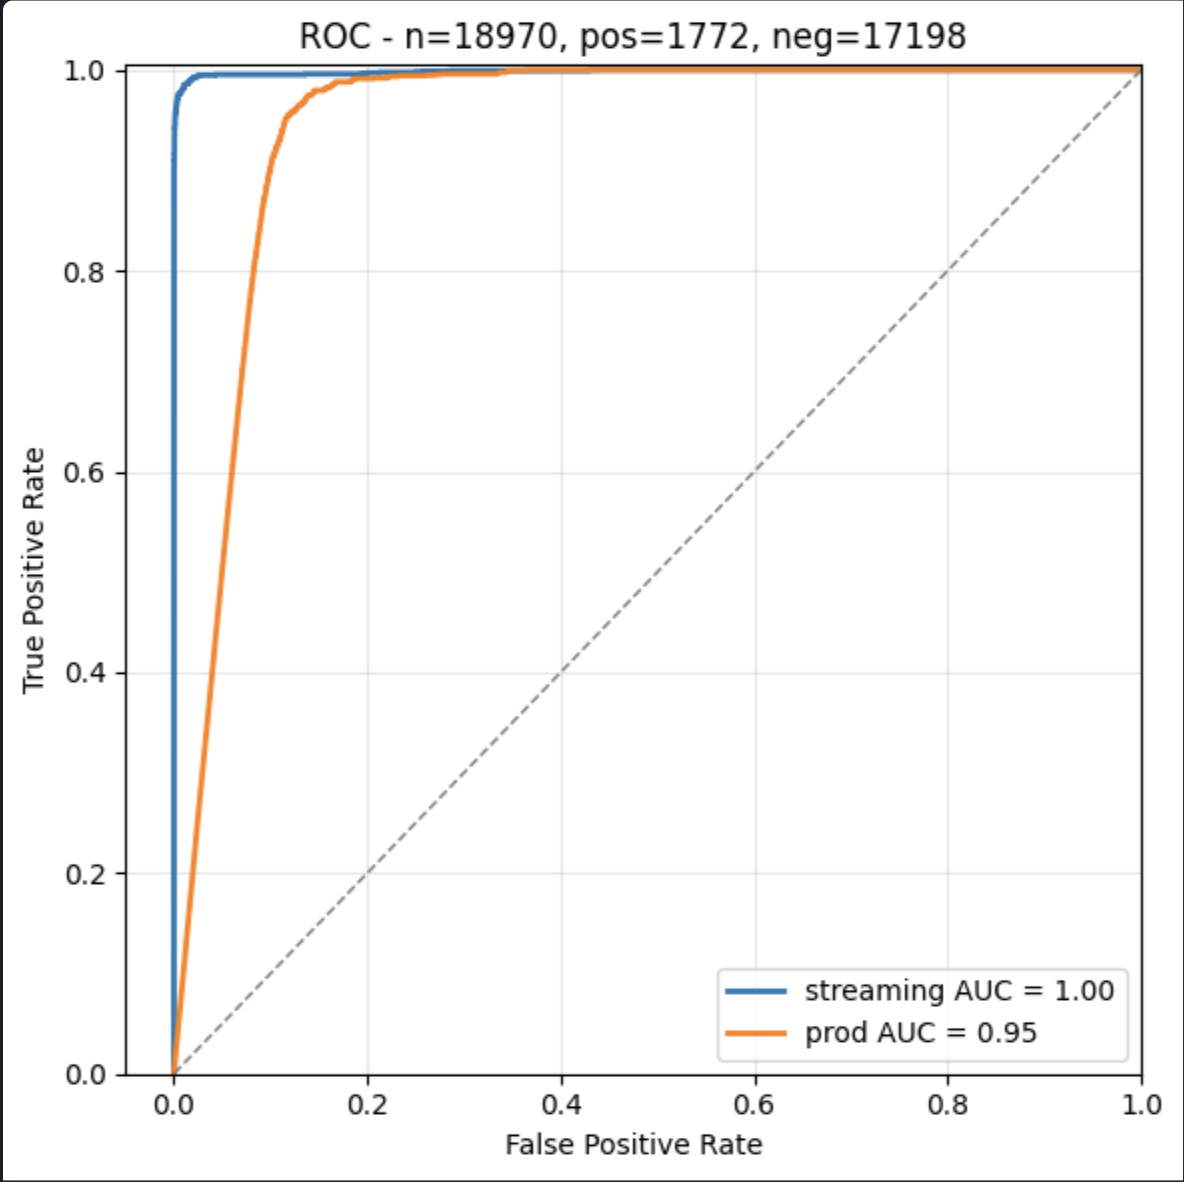
\includegraphics[width=\textwidth]{chapters/figures/censor_old_test.png}
        \caption{Исходный набор (разметка по запросу).}
        \label{fig:sp_censor_old}
    \end{subfigure}

    \vspace{1.5em}

    \begin{subfigure}{0.62\textwidth}
        \centering
        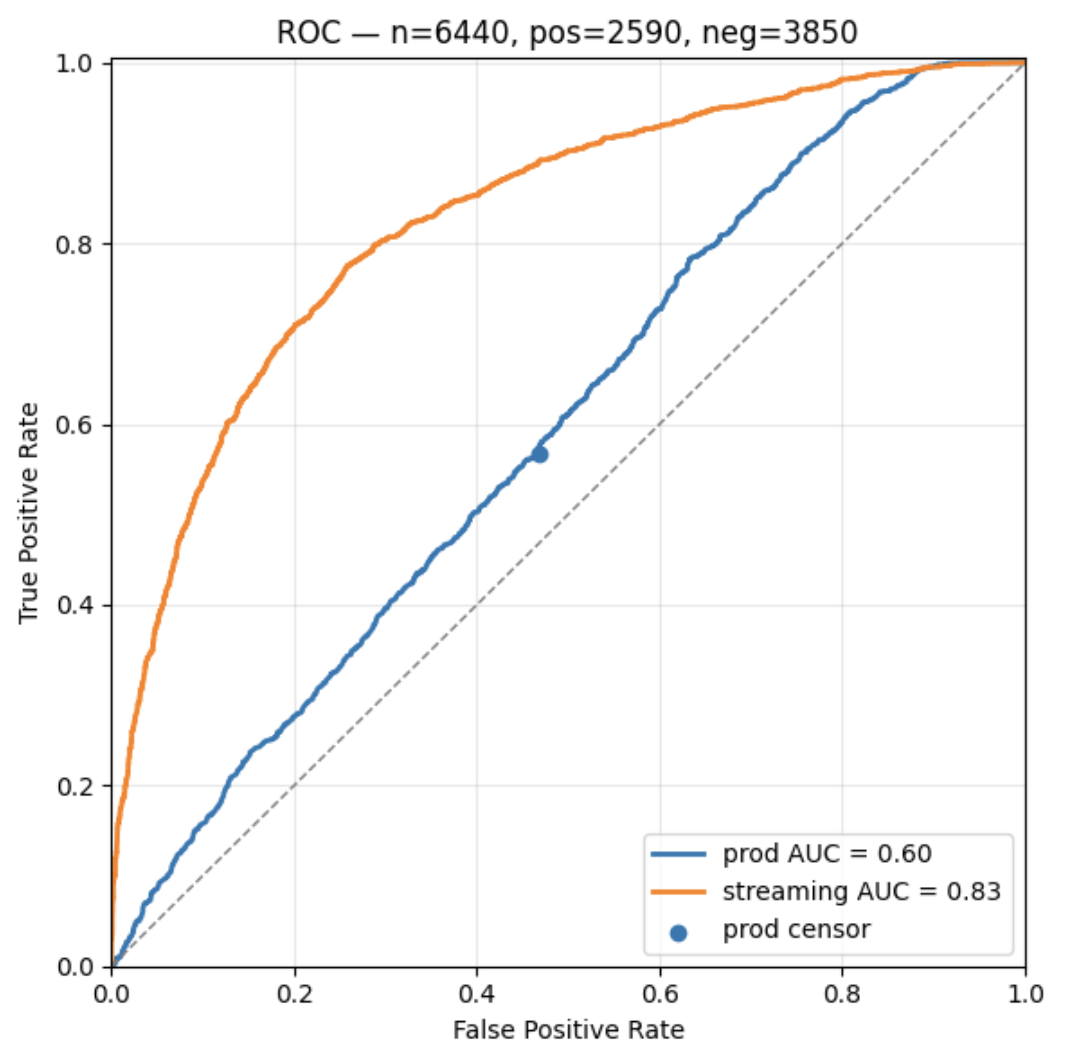
\includegraphics[width=\textwidth]{chapters/figures/censor_new_test.png}
        \caption{Пересмотренный набор (разметка по безопасности ответа).}
        \label{fig:sp_censor_new}
    \end{subfigure}
    \caption{ROC-кривые классификатора запросов (prod) и потокового классификатора ответа (streaming) на исходном и пересмотренном тестовых наборах. Переход к разметке по фактической безопасности ответа выявляет несостоятельность модерации на уровне запроса.}
    \label{fig:sp_censor_roc}
\end{figure}

Рисунок~\ref{fig:sp_censor_roc} сопоставляет ROC-кривые продакшен-классификатора запросов (prod) и потокового классификатора ответа (streaming) на обоих наборах.
На исходном наборе (Рисунок~\ref{fig:sp_censor_old}; $n = 18\,970$, из них $1\,772$ небезопасных и $17\,198$ безопасных обменов) оба классификатора демонстрируют высокое качество --- $\mathrm{AUC} = 0.95$ для классификатора запросов и $\mathrm{AUC} = 1.00$ для потокового, --- что маскирует слабость модерации на уровне запроса.
На пересмотренном наборе (Рисунок~\ref{fig:sp_censor_new}; $n = 6\,440$, из них $2\,590$ небезопасных и $3\,850$ безопасных) качество классификатора запросов падает до $\mathrm{AUC} = 0.60$, приближаясь к случайному угадыванию: его рабочая точка при производственном пороге лежит вблизи диагонали (доля верных обнаружений $\approx 0.57$ при доле ложных срабатываний $\approx 0.47$).
Потоковый классификатор ответа при этом сохраняет существенно более высокую различающую способность ($\mathrm{AUC} = 0.83$).
Полученный разрыв подтверждает, что присвоение метки безопасности обмену, а не изолированному запросу, необходимо для надёжной фильтрации, и обосновывает выбор потоковой классификации ответа в качестве первого этапа конвейера.

Следует подчеркнуть, что, за исключением представленного выше сравнения классификаторов, приведённые в проектной документации значения являются целевыми ориентирами; систематические измерения конвейера в целом составляют предмет дальнейшей работы.

%% =================================================================
\section{Выводы}\label{sec:sp_conclusions}
%% =================================================================

В настоящей главе представлен двухэтапный конвейер обеспечения безопасности мультимодальных больших языковых моделей.
Первый этап --- потоковый классификатор обменов на основе модели GigaChat-10B с архитектурой Mixture of Experts --- выполняет генеративную оценку вредоносности с двухпороговым правилом решения, обеспечивая низкую задержку и независимость от защищаемой модели, и расширяется на визуальную модальность.
Второй этап --- безопасная модель, дообученная методом конституционного ИИ и обучения с подкреплением с гибридной наградой за безопасность, --- формирует неуклончивые ответы, сохраняя баланс между безопасностью и полезностью.
Ключевым элементом конвейера является инструмент безопасного поиска по курируемому индексу, объединяющий поисковый стек, развитый в Главах~\ref{ch:gigaembeddings}--\ref{ch:rag}, с системой обеспечения безопасности и обеспечивающий защищённой модели актуальный и достоверный взгляд на предметную область.


\chapter*{Заключение}
\addcontentsline{toc}{chapter}{Заключение}

В настоящей диссертации разработаны методы информационного поиска для русскоязычных больших языковых моделей и предложена их интеграция в систему обеспечения безопасности мультимодальных моделей. Сквозная линия работы --- от поискового стека к безопасному индексу и далее к двухэтапному конвейеру безопасности --- объединяет извлечение достоверной информации с механизмами модерации контента в единую систему.

\textbf{Основные результаты.} В ходе работы получены следующие результаты.
\begin{enumerate}
    \item Систематизированы современные подходы к построению текстовых и мультимодальных эмбеддингов, методам переранжирования, парадигмам генерации с извлечением информации, а также к системам обеспечения безопасности и уязвимостям мультимодальных моделей (Глава~\ref{ch:lit_review}).
    \item Представлен фреймворк GigaEmbeddings: иерархический трёхэтапный конвейер инструктивного дообучения декодерной LLM GigaChat-3B с двунаправленным вниманием и латентным пулингом. Модель занимает первое место на русскоязычном бенчмарке MTEB(rus, v1.1) со средним баллом 74.16, превосходя сильные базовые модели с большим числом параметров (Глава~\ref{ch:gigaembeddings}).
    \item Предложен кросс-энкодер реранкер на основе компактных декодерных моделей GigaChat-0.6B и GigaChat-3B, адаптирующий декодер в реранкер заменой каузального внимания на двунаправленное, агрегацией mean pooling и выделенной классификационной головой. На трёх русскоязычных IR-бенчмарках реранкер GigaChat-3B достигает наилучшего качества среди открытых моделей сопоставимого размера (Глава~\ref{ch:reranking}).
    \item Построен двухэтапный поисковый стек, объединяющий лексический (BM25), плотный, гибридный и двухэтапный поиск, и обоснованы преимущества RAG в части снижения галлюцинаций и устранения необходимости переобучения при обновлении данных (Глава~\ref{ch:rag}).
    \item Разработан двухэтапный конвейер обеспечения безопасности мультимодальных моделей, включающий потоковый классификатор обменов на основе MoE-модели GigaChat3.1-10B-A1.8B и безопасную модель, дообученную методом конституционного ИИ и обучения с подкреплением с гибридной наградой за безопасность. Поисковый стек интегрирован в конвейер в виде инструмента безопасного поиска по курируемому индексу (Глава~\ref{ch:safety}).
\end{enumerate}

\textbf{Ключевой методологический вывод.} Эмпирически (Глава~\ref{ch:safety}) показано, что присвоение метки безопасности обмену в целом, а не изолированному запросу, необходимо для надёжной фильтрации: при переходе к разметке по фактической безопасности порождённого ответа качество классификатора запросов падает до уровня, близкого к случайному ($\mathrm{AUC} = 0.60$), тогда как потоковый классификатор ответа сохраняет существенно более высокую различающую способность ($\mathrm{AUC} = 0.83$). Этот результат обосновывает выбор потоковой классификации обмена в качестве первого этапа конвейера.

\textbf{Ограничения.} Эмпирически валидированными результатами автора являются модель эмбеддингов (Глава~\ref{ch:gigaembeddings}), реранкер (Глава~\ref{ch:reranking}, со-руководство), сравнение схем классификатора безопасности и конструкция награды (Глава~\ref{ch:safety}). Конвейер безопасности является мультимодальным по построению: потоковый классификатор оценивает изображения, вызовы инструментов и текст, а защищаемая модель обрабатывает изображения, использует режим рассуждения и обращается к инструменту безопасного поиска для запросов любой модальности. Вместе с тем сквозная количественная оценка конвейера в целом --- доля блокировок и чрезмерных отказов, доля высокорисковых уязвимостей, бюджет задержки защитного слоя --- на русскоязычных и мультимодальных бенчмарках безопасности выходит за рамки настоящей работы и составляет предмет дальнейших исследований.

\textbf{Направления дальнейших исследований.} Перспективными представляются: сквозная экспериментальная валидация мультимодального конвейера безопасности на русскоязычных и мультимодальных бенчмарках безопасности (доля блокировок, доля чрезмерных отказов, доля высокорисковых уязвимостей); измерение сквозного бюджета задержки защитного слоя; а также распространение предложенной адаптации декодерных моделей (двунаправленное внимание, mean pooling, классификационная голова) на смежные задачи обработки естественного языка.


\clearpage
\addcontentsline{toc}{chapter}{Список литературы}
\printbibliography

\end{document}
